\documentclass[a4paper, twosided]{book}
\usepackage{CustomStyle}

\begin{document}

\title{}
\begin{titlepage}
    \vspace*{\fill}
    \begin{flushleft}
        \fontsize{50}{10}\selectfont{\textbf{\ttfamily \color{poliOrange} MTQR}}
        \vspace{0.5cm}
        \newline
        \LARGE{\textbf{\ttfamily \color{poliOrange} M\color{poliDarkBlue}onomial %
                                 \color{poliOrange} T\color{poliDarkBlue}ransformation % 
                                 \color{poliOrange}Q\color{poliDarkBlue}uadrature %
                                 \color{poliOrange}R\color{poliDarkBlue}ule}}
    \end{flushleft}
    \vspace{6cm}
    \begin{center}
         \fontsize{40}{10}\selectfont{\textbf{\ttfamily \color{poliDarkBlue}USER MANUAL}}
    \end{center}
    \vspace{0.25cm}
    \begin{center}
         \fontsize{20}{10}\selectfont{\textbf{\ttfamily \color{poliDarkBlue}Installation, integration and execution}}
    \end{center}
    \vspace{10cm}
    
    $\hspace{-2.5cm}\vcenter{
\includegraphics[width=0.6\textwidth]{images/Logo.png}}%
    \hspace{-7.5cm}\vcenter{\begin{minipage}{0.5\textwidth}
        \large{\textbf{\ttfamily \color{poliDarkBlue} Guido Lombardi, PhD,\\ \color{poliOrange}\underline{guido.lombardi@polito.it}}}\\
     \large{\textbf{\ttfamily \color{poliDarkBlue}Davide Papapicco,\\ \color{poliOrange}\underline{davide.papapicco@polito.it}}}
\end{minipage} }$

\end{titlepage}
\frontmatter

\tableofcontents

\mainmatter

\chapter[Preliminaries]{\Huge \ttfamily PRELIMINARIES}\chaptermark{PRELIMINARIES}

This user manual provides a detailed description of the functionalities, correct installation and usage of MTQR, an open-source and cross-platform C++ library for precise numerical integration. Users of the library can refer to the following content for building the static library, as well as integrating it in their own custom applications to generate specialised quadrature rules for integrand functions that can be modelled by sets of singular and generalised polynomials. The principles behind the implementation of the software are discussed in this first Chapter, followed by instructions for compiling and linking the library in Windows and Linux (outlined in the second and third Chapter) and finally by a concluding Chapter that briefly describes the user interface. MTQR offers a high degree of flexibility concerning its usage and interaction, specifically:
\begin{itemize}
    \item it provides high-precision quadrature rules (see Section \ref{Sec2.4}) for multiple applications in numerical mathematics and scientific computing whenever sets of  functions that can be modelled by singular and generalised polynomials require to be integrated;
    \item it implements two {\itshape modes} of execution (namely the {\itshape loud} and {\itshape silent} modes) providing the options of both limiting the terminal's output information and output results (see Section \ref{Sec3.2}) and accelerating and simplifying the overall workflow (see Section \ref{Sec3.2.bis});
    \item it can be deployed as a supporting utility to generate, export and manipulate the new optimised samples and weights for a given set of singular and generalised polynomials (see Section \ref{Sec3.4}).
\end{itemize}
Being a mathematical software, a solid grasp of various topics in mathematical and numerical analysis is an advantage for the user in order to fully exploit the library. In the second Section of this Chapter we provide a brief coverage on some of those concepts such as interpolatory quadrature formulae, Gaussian quadrature rules and asymptotic error estimation which are useful for a full comprehension of the proposed algorithm. Those are followed by the introduction of the monomial transformation, constituting the innovative core of the algorithm and the library, and its properties for quadrature of functions that can be modelled by singular and generalised polynomials. This overview is far from complete and self-contained, and we direct to \cite{Lombardi09, Lombardi21}, and references therein, as the primary sources for a thorough theoretical exposition on the mathematical foundations of MTQR as well as on generalised polynomials (also known as \color{poliDarkBlue} \textbf{Müntz polynomials} \color{black}, see Section \ref{SubSec1.2.4}).

\section[Overview]{\changefont OVERVIEW}\sectionmark{OVERVIEW}\label{Sec1.1}

\noindent
MTQR provides a framework for the high-precision numerical computation of definite integrals whose integrands are functions that can be modelled by singular and generalised polynomials, i.e. whose monomial terms have real degree strictly greater than -1. First and foremost one has to understand the motivation for such library to exist, in order to effectively decide whether or not its usage is necessary for her/his own application. Different techniques have been proposed to numerically approximate singular integrals however the accuracy of their performances is limited by their computational cost, effectively reducing their applications to canonical cases. Another motivation is the possibility to anticipate the required machine-precision in designing the quadrature for a given set of singular and generalised polynomials avoiding to resort to adaptive methods. We wrote MTQR with the aim of helping the user when both singular or generalised polynomials and high precision quadrature are a requirement thus avoiding to compromise between accuracy and time of execution. The pivot algorithm around which the library has been built (i.e. the monomial transformation) has its roots in the relative error estimation of the Gauss-Legendre (G-L) quadrature rule and on the ad-hoc numerical manipulation of the integration parameters \cite{Lombardi21} according to the characteristics of the set of generalised polynomials to be integrated. The combination of those strategies results in an optimized \color{poliDarkBlue} \textbf{monomial transformation quadrature rule} \color{black} that achieves precise numerical integration of singular, generalised polynomials. The background theory of the method refers to \cite{Lombardi09} while this work reports the automatised implementation and performance of the library. The monomial transformation quadrature rule is a result of the application of a novel exact asymptotic error estimate of the G-L quadrature rules that shows the potentialities of such formulae to integrate generalized polynomials composed by monomials of real degree. These characteristics allows to define a  target relative error for sets of generalised monomials (see IEEE floating-point formats' machine-epsilon in Table \ref{table1.1}). Moreover, it enables the extension of the quadrature capability  \color{poliDarkBlue} \textbf{(range of validity)} \color{black} through the use of monomial transformations applied to arbitrary generalised polynomials and in particular to those characterised by an end-point singularity in the integration interval. We want to emphasize these features of MTQR right at the start of this user manual so that the user has a clear understanding of the contexts in which it becomes necessary. In fact, as shown in the test drivers (see Section \ref{Sec2.4}), MTQR significantly outperforms the classical G-L quadrature rule for polynomials whose exponents' sequence is composed of either rational or irrational numbers (henceforth referred to as \color{poliDarkBlue} \textbf{Müntz sequence}\color{black}, see Sub-Section \ref{SubSec1.2.4}). To consistently achieve such performance, our package implements a routine based on the following fundamental steps (discussed in more detail in the second Chapter of this manual):
\begin{enumerate}
    \item select a fixed threshold for the relative error of the integration rule (e.g. the machine-epsilon in IEEE double precision);
    \item exploit the in-depth error estimation of the G-L quadrature to determine the lower and upper bound for the degrees associated to generalised monomials whose quadrature is within the prescribed relative error;
    \item design the monomial transformation to generate a quadrature rule that obtains the specified relative precision on a selected family of generalized polynomials by exploiting the properties of error estimation.
\end{enumerate}

\noindent
Whilst the proposed software certainly allows for the integration of classical monomials and polynomials of integer degree, we remark that these integrands are not the cases for which the library was written (interpolatory classical and generalised Gaussian rules do suffice). Indeed, the core aim of the library is the efficient and precise integration of sets of generalised polynomials where other techniques may require heavy computational cost at run-time \cite{Gautschi94}, or may result in specialized quadratures \cite{Ma1996,Milovanovic2015}. MTQR is entirely written in C++17; beside the speed and versatility of the language, the primary motivation behind such choice was the accessibility to other open-source packages (see Section \ref{Sec2.1}). These packages are essential for the implementation of different routines since they extract fundamental information for the precise quadrature of singular and generalised polynomial integrals. One such example is the ability of handling operations in \textsl{higher-than-double} floating-point arithmetic (e.g. IEEE quadruple floating-point format or higher, see Table \ref{table1.1} below), provided in the \color{poliDarkBlue} \textbf{Boost's Multiprecision} \color{black} library, to secure the precise computation of the quadrature parameters and the quadrature itself. MTQR implements methods that suit a very specific demand in numerical analysis so we used a procedural/modular approach in its writing (as opposed to an object-oriented paradigm) in which all the different functions are hidden behind the library's access point \colorbox{poliGrayBlue}{mtqr} \color{black} module (see Section \ref{Sec2.1} and \ref{Sec2.2}).

\begin{table}[H]
\centering
\begin{tabular}{|c||c|c|c|}
\hline
\multicolumn{4}{|c|}{\textbf{Floating-point formats}} \\
\hline
\textbf{Common name (official)} & \textbf{single (binary32)} & \textbf{double (binary64)} & \textbf{quadruple (binary128)} \\
\hline
\textbf{n. bits}                & 32          & 64           & 128          \\
\textbf{n. decimal digits}      & 7           & 16           & 34           \\
\textbf{epsilon}                & 1.1921 e-07 & 2.2204 e-16  & 1.9259 e-34  \\
\textbf{real min}               & 1.1755 e-38 & 2.2251 e-308 & 3.362 e-4932 \\
\textbf{real max}               & 3.4028 e+38 & 1.7977 e+308 & 1.190 e+4932 \\
\hline
\end{tabular}
  \caption{Some parameters of the most common floating-point formats specified by the IEEE 754 standard \cite{IEEE754}.}
  \label{table1.1}
\end{table}

\newpage
\section[Mathematical background]{\changefont MATHEMATICAL BACKGROUND}\sectionmark{MATHEMATICAL BACKGROUND}\label{Sec1.2}

\noindent
Given a function $f:(a,b)\to\mathbb{R}$, which approximates a target arbitrary integrand with a set of singular and generalised polynomials, we consider its definite integral over the generic integration interval $(a,b)\subset\mathbb{R}$

\begin{equation}\label{eq1.1}
    I(f):=\int_{a}^{b}f(x)dx\,.
\end{equation}

\noindent
The driving purpose of MTQR is to compute a precise numerical approximation of I(f). It is customary to refer to polynomials characterised by natural integer degree $k\in\mathbb{N}$, however our library purposely extends such definition to work with the larger sub-space of generalised polynomials of non-integer (real) degree, i.e. $f\in\mathbb{P}_{\alpha}[x]$ , $\alpha\in(-1,+\infty)$. Of course the analytic integration of polynomial functions is trivial, always leading to an exact form (polynomial) of the primitive $\tilde{f}$ to be evaluated on the integration bounds

\begin{equation}\label{eq1.2}
    I(f) = \Big[\tilde{f}(x)\Big]_{x=a}^{x=b}\,,\quad\tilde{f}\in\mathbb{P}_{\alpha+1}[x], \;\forall f\in\mathbb{P}_{\alpha}[x]\,.
\end{equation}

\noindent
However there are several cases in numerical and computational mathematics in which those integrals are required to be calculated numerically; one such instance are Galerkin methods of approximation of partial differential equations (PDEs) where the local weak formulation of the model requires the numerical evaluation of polynomial integrands modelling some products of the elemental basis functions (e.g. in the Finite and Boundary Element Methods). In famously distinguished applications in scientific computing (e.g. in computational electromagnetics, CEM) non-classical generalised polynomials are used in order to model basis functions featuring an endpoint singularity in either or both the bounds of integration, which cannot be represented exactly or with sufficient accuracy when modelled through regular high-order polynomials  \cite{Graglia04,Graglia08}.

\subsection[Interpolatory quadrature]{\changefont INTERPOLATORY QUADRATURE}\label{SubSec1.2.1}

In order to introduce the topic, we let $f:(a,b)\to\mathbb{R}$ to be any sufficiently regular function; we want to compute $I(f)$ although unfortunately its primitive is not known. One solution is to approximate the function with a polynomial interpolating some of its values at sampled point in $(a,b)$, called \color{poliDarkBlue} \textbf{nodes}\color{black}. Such nodes constitute a finite, countable set $\mathcal{I}_h:=\{x_1\,,\;x_2\,,\;\dots\,,\;x_{n}\}$ which can be thought as a discretisation of the original domain of integration $(a,b)$. The cardinality of such set is  $n$ and it is linked to the degree of the polynomial interpolating $f(x)$; in particular such degree is $n-1$ (i.e. the degree is always equal to the number of nodes minus $1$). The interpolating polynomial $\mathbb{P}_{n-1}\ni\mathcal{L}_{n-1}(x):=\sum_{j=1}^{n}\ell_j(x)f(x_j)$ is expressed in the \color{poliDarkBlue} \textbf{Lagrangian basis} \color{black} whose generators $\ell_j(x)\in\mathbb{P}_{n-1}$ are also polynomials of the same $n-1$ degree. We will not address the theoretical aspects of Lagrangian interpolation and approximation theory since the user may refer to the classical literature about the topic. We can now express the integrand through an approximating polynomial of degree $n-1$

\begin{equation}\label{eq1.3}
    f(x) = \mathcal{L}_{n-1}(x) + E^{'}_n(f) = \sum_{j=1}^{n}\ell_j(x)f(x_j) + E^{'}_n(f)\,\quad x_j\in\mathcal{I}_h\,,\;\forall j=1,...,n\,.
\end{equation}

\color{black}

\noindent
By substituting (\ref{eq1.3}) in (\ref{eq1.1}) we obtain an approximation of the initial integral known as an \color{poliDarkBlue} \textbf{interpolatory quadrature formula} \color{black}

\begin{equation}\label{eq1.4}
    I(f) = \int_a^b (\mathcal{L}_{n-1}(x) + E^{'}_n(f))\,dx = \sum_{j=1}^{n}f(x_j)\int_a^b \ell_j(x)\,dx + \int_a^b E^{'}_n(x) = \sum_{j=1}^{n}w_j\,f(x_j) + E_n(f)\,,
\end{equation}

\noindent
where we define the \color{poliDarkBlue} \textbf{weights} \color{black} $w_j$ of the quadrature formula as the definite integral of the Lagrangian basis' generators and the \color{poliDarkBlue} \textbf{remainder} \color{black} as $E_n(f):=\int_a^b E^{'}_n(f)\,dx$. It is a well known result in numerical analysis that any interpolatory quadrature rule made on $n$ samples is exact, i.e. $E_n(f)=0$, if the integrand is any polynomial of degree up to $n-1$.

\subsection[Gaussian quadrature formulae]{\changefont GAUSSIAN QUADRATURE FORMULAE}\label{SubSec1.2.2}

One of the main issues with numerical integration using interpolatory quadrature is the selection of the nodes' distribution. The simplest case is the uniformly distributed partition 
$\mathcal{I}_h =\big\{x_j = a + (j-1)\,h\,,\;h:=\frac{b-a}{n}\big\}_{j=1,...,n}$ which results in the \color{poliDarkBlue} \textbf{Newton-Cotes quadrature formula}\color{black}. As reported in the classical literature, better choices for such distribution, depending on the properties and behaviour of $f(x)$, are available. In particular the \color{poliDarkBlue} \textbf{Gaussian quadrature formula} \color{black} is one where each of the nodes uniquely corresponds to the root of an orthogonal polynomial. To introduce these approximations we now let the integrand to be an arbitrarily regular function

\begin{equation}\label{eq1.5}
    \mathcal{C}^m[\mathcal{I}]\ni f(x) = w(x)g(x)\,,\quad m\in\mathbb{N}\,,
\end{equation}

\noindent
where the factorised $g(x)$ always contains its most regular part whereas $w(x)$, known as the \color{poliDarkBlue} \textbf{weight function} \color{black} contains, if present, any irregular and/or singular part of $f(x)$. If the weight function is not null everywhere in $(a,b)$ and we can find an infinite sequence of classical polynomials $P:=\big\{p_j(x)\in\mathbb{P}_j\big\}_{j=0,1,...}$ s.t.

\begin{equation}\label{eq1.6}
    \int_a^b w(x)p_j(x)p_k(x)\,dx = \alpha_{jk}\delta_{jk}\,,\quad\forall p_j\,,\;p_k\in P\,,
\end{equation}

\noindent
where $\delta_{jk}$ is the Kronecker delta, then $P$ represents a \color{poliDarkBlue} \textbf{system of orthogonal polynomials} \color{black} w.r.t. the specified weight function $w(x)$. Any Gaussian quadrature formula built on  $n$ nodes is exact for any classical polynomial integrand $g(x)$ of degree up to $2n-1$. It is therefore easy to see why Gaussian quadrature rules are usually preferred over Newton-Cotes formulae when dealing with regular functions with a known, factorised weight $w(x)$. Although Gaussian quadrature allows the exact integration with respect to a limited number of weight functions, throughout the years they have been generalised using refined approximations and numerical efforts \cite{Gautschi94}. The simplest and arguably most widely used Gaussian quadrature rule is the Gauss-Legendre (G-L) formula, for which the sequence $P$ is made of \color{poliDarkBlue} \textbf{Legendre's polynomials} \color{black} that are orthogonal w.r.t. the constant weight function $w(x)=1$ over the interval $(a=-1\,,\;b=+1)$.

\subsection[Asymptotic error estimation]{\changefont ASYMPTOTIC ERROR ESTIMATION \color{black}}\label{SubSec1.2.3}

This Sub-Section analyzes the accuracy of the G-L quadrature formula with $n$ nodes. As reported in the previous Sub-Section, if $f(x)\in\mathbb{P}_k\,,\;k\in\mathbb{N}$ we'd have $E_n(f)=0,\,\forall k\leq2n-1$.  
In analysing the performance of a numerical algorithm it is often more appropriate to define and use an a-posteriori (actual) relative error associated to the approximating techniques, rather than an {\itshape absolute} one s.a. the remainder $E_n(f)$. For the specific case of the numerical integration of an arbitrary function $f(x)$, via a G-L formula, we have
\begin{equation}\label{eq1.7}
    R_n^{(a)}(f) = \frac{|I(f)-I_n(f)|}{|I(f)|}\,,\quad I_n(f):=\sum_{j=1}^{n}w_j\,f(x_j)\,,
\end{equation}
\noindent
where the sequence of pairs $\{(x_j,w_j)\}_{j=1,...,n}$ is the set of nodes and weights of the G-L quadrature rule. In those cases, where the performance of the quadrature rule, in terms of the associated relative error, needs to be known a priori, we must refer to an estimate of (\ref{eq1.7}) 
\begin{equation}\label{eq1.8}
    R_n(f) = \frac{|E_n(f)|}{|I(f)|} \sim R_n^{(a)}(f)\,,
\end{equation}
where $E_n(f)$ is the estimated reminder of the quadrature rule. In \cite{Lombardi09}, one of the authors of the present work, derived a closed form a-priori error asymptotic estimation of $E_n(f)$ for a G-L formula applied to a generalised monomial term $f(x)=x^\lambda$ with real-valued degree $\lambda>-1$.
\begin{equation}\label{eq1.9}
    E_n(x^\lambda) = -2^{-2\lambda}\,\lambda\,\sin(\pi \lambda) \bigg(\frac{B(2\lambda,2n-\lambda)}{2n+\lambda} - \frac{B(2\lambda, 2+2n-\lambda)}{2+2n+\lambda}\bigg)\,,
\end{equation}
\noindent
where $B(z,w):=\frac{\Gamma(z)\Gamma(w)}{\Gamma(z+w)}$ is the Euler's Beta function. This result is important for the development of an ad-hoc quadrature rule whose error can be computed a-priori for any generalised polynomial integrand function. In particular, given a specified number of quadrature nodes $n$, we can clearly see in Figure \ref{Fig1.1} how the a-priori relative error estimate $R_n(x^\lambda)$ behaves asymptotically with $\lambda$. For instance we immediately notice that the value of $R_n(f)$, with a fixed $n$ samples, is below a pre-determined arbitrary precision (in terms of relative error) within a specific, finite range of values of $\lambda$ which we identify as $(\lambda_{\text{min}},\lambda_{\text{max}})\subset(-1,+\infty)$. In practice we can specify a finite-arithmetic threshold, for example the machine-epsilon in double f.p. format as reported in the figure below (see constant black line). Once identified, the interval $(\lambda_{\text{min}}, \lambda_{\text{max}})$ exactly coincides with the real range of exponents of the set of generalised polynomial functions whose numerical integration (using the specified G-L quadrature rule) would be exact in finite arithmetic.

\begin{center}
        \begin{figure}[H]
        \captionsetup{singlelinecheck=off}
        \includesvg[keepaspectratio, width=\textwidth]{images/Fig1_1.svg}
        \caption{Evaluation of the relative error estimate $R_n(x^{\lambda})$ (in logarithmic scale) provided in (\ref{eq1.8}) for $n=10,18,26,34,42$. Notice that for a fixed $n$ we have that $R_n(x^{\lambda})$ is smaller than an arbitrary precision threshold in $(\lambda_{\text{min}},\lambda_{\text{max}})$. Furthermore, as long as $\lambda$ is a natural integer value smaller than $2n-1$, the relative error shows negative spikes, therefore mimicking the property of a G-L quadrature to feature zero reminder. Finally we emphasize that for $n=10$ the estimate barely reaches the machine-epsilon threshold for double precision entailing that it is the minimum number of nodes that can be used to achieve double precision quadrature for a limited range of real $\lambda$.}
        \label{Fig1.1}
        \end{figure}
\end{center}

\subsection[Müntz theorem and generalised polynomials]{\changefont MÜNTZ THEOREM AND GENERALISED POLYNOMIALS }\label{SubSec1.2.4}

In the opening Sub-Section we mentioned that MTQR extends the integration capabilities of the G-L formulae to generalised polynomials of real degree in a selected range of exponents $(-1,+\infty)$ by means of monomial transformations. As the reader may find in \cite{Lombardi09} and references therein, a complete theory on the properties of these kind of functions relates to Müntz polynomials, orthogonal Müntz polynomials and their numerical computation. 
\newline
We assume that the generalized polynomials feature a sequence of (real) exponents that is a subset of a Müntz sequence, i.e. an ordered sequence of real numbers $\Lambda:=\{\dots>\lambda_j>\lambda_{j-1}>\dots>\lambda_1>-1\}$ s.t.

\begin{equation}\label{eq1.10}
    \sum_{j=1}^{+\infty}\frac{1}{\lambda_j}=+\infty\,.
\end{equation}

\noindent
Such condition satisfies the known \color{poliDarkBlue} \textbf{Müntz theorem} \color{black} for which the vector space $\Pi(\Lambda):=\text{span}\{x^{\lambda_j}\}$ spanned by the monomials of degree in $\Lambda$ is dense in $\mathcal{C}(0,1]$. Elements $p^{(m)}(x) = \sum_{j=1}^{r} c_j\,x^{\lambda_j}\in\Pi(\Lambda)$ are therefore known as \color{poliDarkBlue} \textbf{Müntz polynomials} \color{black} of degree $\lambda_r$ defined in $(0,1]$ where  $\Lambda_r:=\{\lambda_r>\dots>\lambda_j>\lambda_{j-1}>\dots>\lambda_1>-1\},\, r\in\mathbb{N}_0$. In the following we shall assume that any polynomial with $r$ terms having at least one constituting monomial of non-integer degree are to be considered Müntz (generalised) polynomials. The monomial transformation quadrature rule implemented in MTQR is capable of approximating the integral of functions modelled by generalised polynomials defined in $(0,1)$ and, crucially, featuring an endpoint singularity at $x=0$. The proposed quadrature allows to obtain an arbitrary fixed precision for the integral combining the G-L quadrature's performance (see in Figure \ref{Fig1.1} the relative error falls below the machine-epsilon threshold in double f.p. format) with an ad-hoc designed monomial transformation by exploiting the properties of error estimation.

\newpage
\subsection[Integration interval]{\changefont INTEGRATION INTERVAL}\label{SubSec1.2.5}

We consider the problem of numerically integrating a function that is approximated appropriately with a set of generalised polynomials in the interval $(a,b)$. This problem can always be reformulated in $(0,1)$ with a potential (endpoint) singularity in $x=0$ via affine transformation, i.e. 
\begin{equation}\label{eq1.11}
    I(f) = \int_0^1 f(\tilde{x}) d\tilde{x}\,.
\end{equation}
This choice is due to:
\begin{itemize}
  \item uniquely investigate the precision property of G-L quadrature and derive unique rules to design a monomial transformation for the numerical integration algorithm;
  \item avoid or at least severely restrict the effects of numerical cancellation in the numerical quadrature of singular generalised polynomials with endpoint singularities other than $x=0$; 
  \item to be consistent with the definition of Müntz polynomials and approximation theory.
\end{itemize}

\noindent
The second property is necessary to avoid rounding errors in the calculation of the transformed quadrature nodes. In fact, as the quadrature points tend to be clustered around the singularity, when it is located far from the origin $x=0$, the resulting samples may be affected by numerical cancellation. Often, in practical problems, integration on an arbitrary interval $(a,b)$ is requested. For this reason, we need to define an affine transformation to map the original, generic, integration interval $(a,b)$ into $(0,1)$. To that purpose, let us introduce a (linear) affine map $\varphi:(a,b)\to(0,1)$ specified as
\begin{equation}\label{eq1.12}
    \varphi(y) := \alpha\,y + \beta = \tilde{x}\,,\quad y\in(a,b)\,.
\end{equation}
\noindent
It is easy to see that $\varphi(y=0)=\beta\equiv a$ and $\varphi(y=1)=\alpha-\beta\equiv b$. We obtain
\begin{equation}\label{eq1.13}
    I(f) = \int_a^b f(y) dy = \int_{0}^{1} f\Big(({b-a})\tilde{x}+a\Big)\,J_{[a,b]}\,d\tilde{x}\,,\quad J_{[a,b]}:=b-a\,.
\end{equation}
\noindent
This new form (\ref{eq1.13}) of the integral can now be computed numerically using the monomial transformation quadrature rule by considering that singular integrands at the endpoint $y=a$ will now have a singularity in $\tilde{x}=0$. The same transformation can be useful to easily map standard G-L quadrature samples and weights $\{y_j, v_j\}_{j=1,...,n}$ defined in $(-1,1)$ to the less common G-L quadrature samples and weights $\{\tilde{x}_j,\tilde{w}_j\}_{j=1,...,n}$ defined in $(0,1)$ which is considered as the starting point to apply the monomial transformation quadrature rule. In this specific case we obtain
\begin{equation}\label{eq1.14}
    I(f) = \int_{-1}^1 f(y) dy =\sum_{j=1}^n f(y_j)v_j = \int_{0}^{1} f\Big(2\tilde{x}-1\Big)\,2\, d\tilde{x}=\sum_{j=1}^n 2\,\tilde{w}_j f(2 \tilde{x}_i-1)\,,
\end{equation}
\noindent
thus
\begin{equation}\label{eq1.15}
    \tilde{w}_j=\frac{v_j}{2}, \;\: \tilde{x}_j=\frac{y_j+1}{2}, \quad j=1,...,n\,.
\end{equation}
\noindent
One important remark is that, once the new sample and weights $\{\tilde{x}_j,\tilde{w}_j\}$ have been derived for the proposed monomial transformation quadrature (the algorithm is described in the following Sub-Section \ref{SubSec1.2.6}), we should avoid to map them back to the original integration interval $(a,b)$ due to numerical cancellation in the representation of the samples near the singular endpoint, say $y=a$. The novel quadrature is therefore safely applied in $(0,1)$ by re-formulating in it the original integration problem defined in $(a,b)$ as done in (\ref{eq1.13}).

\subsection[Monomial transformation]{\changefont MONOMIAL TRANSFORMATION}\label{SubSec1.2.6}

Given a set of Müntz (generalised) polynomials we define $\lambda_{\text{min}}$ and $\lambda_{\text{max}}$ as the smallest and greatest values, respectively, in the Müntz sequence of exponents. From Sub-Section \ref{SubSec1.2.4} we know that $\lambda_{\text{min}}>-1$ (we consider only integrable functions) and refer to $\lambda_{\text{max}}$ as the largest degree of the polynomials. Recall also that only for classical polynomials (i.e. $\lambda_j\in\mathbb{N}$) we obtain $E_n(f)=0$ when using G-L formulae with $n = \lceil \frac{\lambda_{\text{max}}+1}{2} \rceil$ samples. Regardless, generalised singular polynomials, s.a. those in Müntz vector space, are integrated with poor accuracy by classical G-L with a specified number of nodes when containing generalised monomials with integration relative errors beyond the selected threshold. Analysis of (\ref{eq1.8}) and (\ref{eq1.9}) allow to fully exploit the performance of G-L quadrature rule when applied to generalised monomials; specifically they are used to design an ad-hoc monomial transformation $\gamma(\tilde{x}):(0,1)\to(0,1)$, for the set of polynomials identified by $\lambda_{\text{min}}$ and $\lambda_{\text{max}}$
\begin{equation}\label{eq1.16}
    x = \gamma(\tilde{x}) = \tilde{x}^r\,,\quad\tilde{x}\in(0,1)\,,
\end{equation}

\noindent
with the constraint (see derivation in \cite{Lombardi09, Lombardi21})
\begin{equation}\label{eq1.17}
    r_{\text{min}}:=\frac{1+\beta_{\text{min}}(n)}{1+\lambda_{\text{min}}} < r < \frac{1+\beta_{\text{max}}(n)}{1+\lambda_{\text{max}}}=:r_{\text{max}}\,,
\end{equation}

\noindent
where $\beta_{\text{min}}(n)$ and $\beta_{\text{max}}(n)$ are the minimum and maximum exponents for generalised monomial functions that can be integrated with a relative error strictly smaller than a fixed finite precision using G-L quadrature with $n$ samples, see also Figure \ref{Fig1.1}. Given some expression for $(\beta_{\text{min}}(n),\beta_{\text{max}}(n))$ enforcing (\ref{eq1.17}) yields a unique minimum value of $n$ (henceforth referred to as $n_{min}$) that satisfies the above constraint of being the (sole) real root of
\begin{equation}\label{eq1.18}
    (-4.0693\cdot10^{-3}+4.1296\cdot10^{-4}n)[(8.8147+1.0123\cdot10^{-1}n^2)\cdot(1+\lambda_{\text{min}})-(1+\lambda_{\text{max}})]^3 - (1+\lambda_{\text{max}})^3=0\,.
\end{equation}

\noindent
Given $n_{min}$ one can easily compute $r$, for example, as the midpoint between the upper and lower bounds of the inequality in (\ref{eq1.17}) and easily derive new nodes and weights computed, according to \cite{Lombardi09,Lombardi21}, via (\ref{eq1.16}) and 
\begin{equation}\label{eq1.19}
    x_j=\tilde{x}_j^{r},\quad w_j = r\tilde{x}_j^{r-1}\tilde{w}_j\,\quad\forall j=1,...,n\,,
\end{equation}

\noindent
respectively, where $\tilde{x}_j,\:\tilde{w}_j$ are the classical G-L nodes and weights mapped in $(0,1)$.

\begin{center}
        \begin{figure}[h]
        \captionsetup{singlelinecheck=off}
        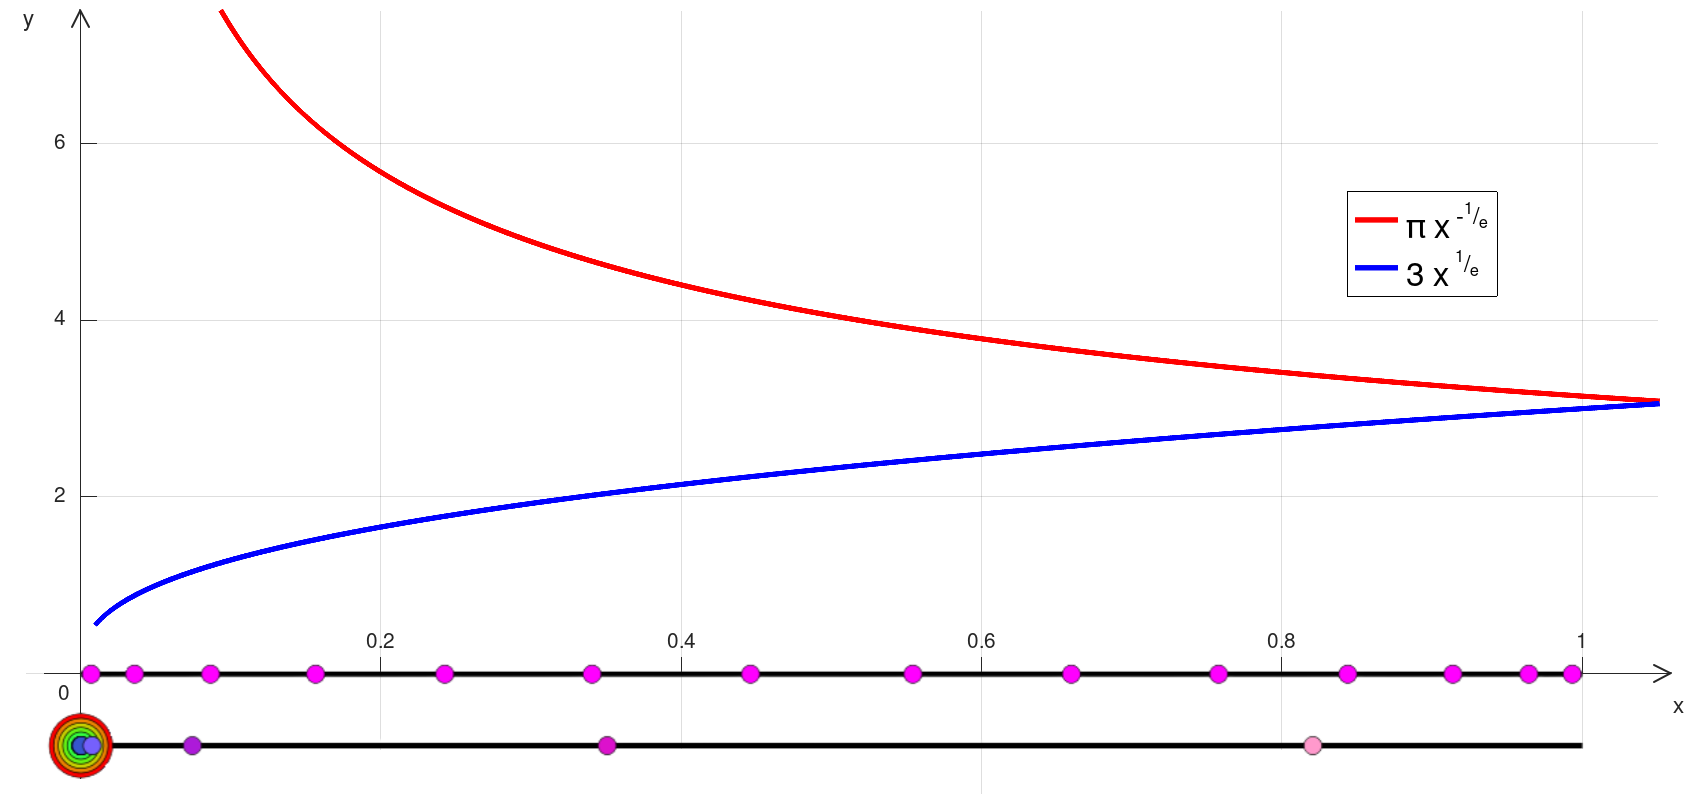
\includegraphics[keepaspectratio,width=\textwidth]{images/Fig1_2.png}
        \caption{Plot of the monomial terms in (\ref{eq1.20}). On the lower part of the graph a distribution in $(0,1)$ of the $n=14$ nodes of a classical G-L formula (magenta) and the new samples obtained by the monomial transformation quadrature rule (linear color gradient) is reported (with double precision threshold for integration). Due to the clustering of the latter they are plotted as scaled-down circles as we move from $x=0$ to $x=1$. Observe how classical G-L nodes in $(0,1)$ are inefficiently organised to capture the singularity in $x=0$. Conversely the action $(\ref{eq1.16})$ (whose order $r=17.5249867$ is given by (\ref{eq1.17})) re-arranges the vast majority of nodes around $x=0$ which is an endpoint singularity for the generalised monomial term $x^{-\frac{1}{e}}$
        and an irregular endpoint for the generalised monomial term $x^{+\frac{1}{e}}$, securing precision for set of polynomials with $\lambda\in (-1/e, + 1/e)$.}
        \label{Fig1.2}
        \end{figure}
\end{center}

\noindent
The transformed new nodes and weights are optimised for the accurate numerical integration in $(0,1)$ of the two monomials with the minimum and maximum exponents, i.e $c_{min}\,x^{\lambda_{\text{min}}}$ and $c_{max}\,x^{\lambda_{\text{max}}}$, guaranteeing the same f.p. precision for any additional monomial term $c\,x^\lambda$ with $\lambda \in (\lambda_{\text{min}},\lambda_{\text{max}})$. For example, consider the following  Müntz polynomial
\begin{equation}\label{eq1.20}
    \Pi(\Lambda)\ni p(x) = \pi x^{-\frac{1}{e}} + 3x^{\frac{1}{e}}\,,\quad\Lambda=\Big\{-\frac{1}{e},\frac{1}{e}\Big\}\,.
\end{equation}

\noindent
A visual representation of $p(x)$ is reported in Figure \ref{Fig1.2} together with the effect of the ad-hoc designed monomial transformation on the quadrature for double precision integration. In this case, the library only uses $n_{min}=14$ quadrature samples for a monomial transformation order $r=17.5249867$ yielding $I_n(f)=7.1631021363408645$ and $E_n(f)=2.2826531409965486\cdot10^{-17}$. We postpone the values of those new nodes and weights in Table \ref{table3.1} at the end of Sub-Section \ref{Sec3.4} where we implemented $(\ref{eq1.20})$ using the library in different modes of execution.

\chapter[Installation]{\Huge \ttfamily INSTALLATION}\chaptermark{INSTALLATION}

In the following Chapter we illustrate how to build executable applications with MTQR as well as the dependencies needed at link-time. We begin from the latter topic by outlining the third-party packages necessary for the library prior to the compilation itself. Later, a brief description of the organisation and structure of the code is given in order to facilitate the comprehension of the user interface. Then, we explain how to build the library itself and finally illustrate its core features by running testing applications shipped with the software. We postpone to the next Chapter a description of the two {\itshape modes} of execution, namely the \color{poliDarkBlue} \textbf{loud} \color{black} and \color{poliDarkBlue} \textbf{silent mode} \color{black}.

\section[Dependencies]{\changefont DEPENDENCIES}\sectionmark{DEPENDENCIES}\label{Sec2.1}

\noindent
As reported in the opening Section, MTQR is entirely written in C++17; besides the speed and versatility of the language, the primary motivation behind such choice was the accessibility to other open-source mathematical packages. Indeed MTQR relies on two libraries that are well-known in the scientific computing and open-source communities listed below:

\begin{itemize}
    \item \color{poliDarkBlue} \textbf{Boost C++ libraries} \color{black}\cite{boost}: a vast, peer-reviewed, collection of mostly header source files. In particular MTQR extensively uses the \colorbox{poliGrayBlue}{Multiprecision} library, where non-native higher precision f.p. formats have been implemented as C++ data-types. In particular the library depends on the \colorbox{poliGrayBlue}{cpp\_bin\_float} back-end, and more specifically the \colorbox{poliGrayBlue}{cpp\_bin\_float\_quad} number type (henceforth referred to as \colorbox{poliGrayBlue}{float128}) is used as a drop-in replacement of C++ f.p. native data types to efficiently implement IEEE 754 quadruple precision across multiple architectures and compilers\footnote{We deployed \colorbox{poliGrayBlue}{float128} only to secure the precise computation of the quadrature parameters and the quadrature itself in the most computationally demanding cases.};
    
    \item \color{poliDarkBlue} \textbf{GSL - GNU Scientific Library} \color{black}\cite{gsl}: required by MTQR in only one instance, that is the computation of the roots of $(\ref{eq1.18})$ via the method \colorbox{poliGrayBlue}{gsl\_poly\_complex\_solve}. Alternative solvers and root-finders are available however in our case we were also interested in automatically locating the sole real root of such polynomial (corresponding to $n_{\text{min}}$ in $(\ref{eq1.18})$), hence the choice we made.
\end{itemize}

\noindent
The user must make sure that both libraries are correctly installed on the local system and that they are either placed in the default search paths of the user's preferred C++ compiler and linker or that the appropriate environment variable is amended according to the desired location of the source code of the aforementioned libraries. Platform-specific instructions are outlined in the following Sub-Section for correctly installing and placing both the aforementioned dependencies as well as the building tools (\color{poliDarkBlue} \textbf{CMake} \color{black} and \color{poliDarkBlue} \textbf{GNU make} \color{black}) needed to correctly compile MTQR in Linux and Windows. We remark that the installation and build of the library and all its dependencies has been tested on multiple combinations of OS and C++ compilers as reported in Table \ref{table2.1}.

\begin{table}[H]
\centering
\begin{tabular}{|c||c|c|c|c|c|c|c|}
\hline
\multicolumn{8}{|c|}{\textbf{Platform combinations}} \\
\hline
Env. n. & OS & Processor & Compiler & Make & CMake & Boost & GSL \\
\hline
1 & Ubuntu 22.04.1 & Intel Core i5-6300U @ 3.0 GHz & GCC 11.3.0 & 4.3.0 & 3.21.1 & 1.74 & 2.7 \\
2 & Ubuntu 20.04.3 & Intel Core i5-1035G1 @ 1.0 GHz & GCC 9.3.0 & 4.2.1 & 3.20.2 & 1.77 & 2.5 \\
3 & CentOS 8.5 & Intel Core i7-10700 @ 2.9 GHz  & GCC 8.5.0 & 4.2.1 & 3.20.4 & 1.66 & 2.5 \\
4 & Windows 11 & Intel Core i7-10700 @ 2.9 GHz  & MVSC 14.32 & N/A & 3.25.4 & 1.81 & 2.7 \\
5 & Windows 11 & AMD Ryzen 7 5875U @ 2.0 GHz & MVSC 14.34 & N/A & 3.25.2 & 1.81 & 2.7 \\
\hline
\end{tabular}
  \caption{Tested development environments.}
  \label{table2.1}
\end{table}

\subsection[Linux]{\changefont LINUX}\label{SubSec2.1.1}

The proper installation of all the dependencies required by MTQR in Linux is straightforward thanks to package managers s.a. the \color{poliDarkBlue} \textbf{advanced package tool} \color{black} or \color{poliDarkBlue} \textbf{yellowdog updater modified} \color{black} (based on the user's distro). The user shall run the following commands on the terminal and verify the correct installation by checking their version\footnote{CentOS Linux 8 has reached the EOL at the end of 2021. To update it you need to change the mirrors to \color{poliDarkBlue} \textbf{vault.centos.org} \color{black} where they are permanently archived (see https://techglimpse.com/failed-metadata-repo-appstream-centos-8). CentOS Linux 9 requires the installation of gsl-devel via 
\colorbox{poliGrayBlue}{sudo dnf install http://mirror.stream.centos.org/9-stream/CRB/x86\textunderscore64/os/Packages/gsl-devel-2.6-7.el9.x86\textunderscore64.rpm}. In some Linux distros, s.a. Ubuntu 22.04, CMake cannot find PkgConfig; please proceed with \colorbox{poliGrayBlue}{sudo apt-get install --reinstall pkg-config cmake-data}.}.

\vspace{0.2cm}
\begin{tcblisting}{enhanced,
                   arc=5mm,
                   title = \color{black}{\large \ttfamily Installation of third-party libraries (Linux)},
                   colbacktitle=bashGray,
                   colback=bashBlue,
                   listing only,
                   listing style=BashStyle}
# For Debian-based distros (Ubuntu, Mint, Knoppix, Kali ...)
user@machine: home> sudo apt-get update
user@machine: home> sudo apt-get install build-essential libboost-all-dev libgsl-dev cmake
user@machine: home> gcc --version
user@machine: home> make --version
user@machine: home> cmake --version
# For RPM-based distros (CentOS, Fedora, SUSE, Scientific Linux ...)
user@machine: home> sudo dnf makecache --refresh
user@machine: home> sudo dnf install http://repo.okay.com.mx/centos/8/x86_64/release/okay-release-1-1.noarch.rpm
user@machine: home> sudo dnf install gcc gcc-c++ make cmake
user@machine: home> sudo dnf install boost gsl libquadmath
user@machine: home> sudo dnf install boost-devel gsl-devel
user@machine: home> gcc --version
user@machine: home> make --version
user@machine: home> cmake --version
\end{tcblisting}
\vspace{0.3cm}

\noindent
Notice that in the above lists of terminal commands we installed both \color{poliDarkBlue} \textbf{CMake} \color{black} and \color{poliDarkBlue} \textbf{make}\color{black}. This is because, while the preferred and de-facto standard building tools used to compile C++ libraries is \colorbox{poliGrayBlue}{cmake}, on Linux we decide to allow the users to have the additional option of building MTQR also using only \colorbox{poliGrayBlue}{make}. For more information on how MTQR allows using Make for compiling the library we redirect on Sub-Section \ref{SubSec2.3.1}.

\subsection[Windows]{\changefont WINDOWS}\label{SubSec2.1.2}

Installation of the dependencies in Windows\footnote{For a smooth setup, we suggest to install Microsoft Visual Studio (we tested v. 2022) with default packages and C++ Desktop Applications support. We also recommend to install Git (https://git-scm.com/, we tested v. 2.41.0), for \color{poliDarkBlue} \textbf{vcpkg} \color{black} package manager.} is somewhat more cumbersome when compared to Linux; we report the simplest and most secure installation of the third-party packages to achieve a successful build of MTQR:

\begin{itemize}
   \item GSL can be installed via the \color{poliDarkBlue} \textbf{vcpkg} \color{black} package manager which is downloaded using \color{poliDarkBlue} \textbf{Windows PowerShell}\color{black}; we recommend the root directory as installation path since this facilitates the setup for the user. The procedure for a correct installation and set up for these dependencies is reported below;

    \item one of the most practical features of Boost's libraries is that they are (mostly) made by header files which do not need to be compiled; MTQR's dependency on Boost is restricted to the Multiprecision library. The user shall download the archived \colorbox{poliGrayBlue}{boost\_1\_81\_0.7z or .zip}  file from the official Boost v1.81.0 release \cite{boost_release}, decompress it in a folder named \colorbox{poliGrayBlue}{boost} and place it in the \colorbox{poliGrayBlue}{C:\textbackslash} root directory. This way the user is sure that \colorbox{poliGrayBlue}{CMake} can find Boost headers and properly include them in the MTQR's source code;

    \item on Windows MTQR can only be compiled using \color{poliDarkBlue} \textbf{CMake}\color{black}. The easiest and safest procedure of installing CMake on Windows is by downloading the binaries from the original webpage and running the installer\footnote{We advise to select the option to include it in the path and then restart the OS.}.
\end{itemize}

\noindent
In our build we used Microsoft Visual Studio 2022 which automatically runs \colorbox{poliGrayBlue}{CMake} in any directory containing a \colorbox{poliGrayBlue}{CMakeLists.txt} and, if successful, autonomously creates the associate project files (see Sub-Section \ref{SubSec2.3.2}).
\vspace{0.15cm}
\begin{tcblisting}{enhanced,
                    arc=5mm,
                    title = \color{black}{\large \ttfamily Installation of third-party libraries (Windows)},
                    colbacktitle=bashGray,
                    colback=black,
                    listing only,
                    listing style=PSStyle}
PS C: > git clone https://github.com/Microsoft/vcpkg.git
PS C: > cd .\vcpkg\
PS C: > .\bootstrap-vcpkg.bat
PS C: > .\vcpkg.exe integrate install
PS C: > .\vcpkg.exe install gsl gsl:x64-windows
PS C: > .\vcpkg.exe list
PS C: > cmake --version
\end{tcblisting}
\vspace{-0.2cm}

\subsection[Integration]{\changefont INTEGRATION}\label{SubSec2.1.3}

\noindent
The dependencies are constituted of large libraries, although MTQR uses a limited amount of the methods they provide. We therefore made sure that only the necessary parts of the libraries are included in the source code, striving to maintain a clean and light final product. This is evidenced in the content of the library's principal header file \colorbox{poliGrayBlue}{mtqr.h} which is reported in the snippet below.

\vspace{0.15cm}
\tcbinputlisting{enhanced,
                 arc=5mm,
                 title = \color{black}{\large \ttfamily mtqr.h},
                 colbacktitle=poliOrange,
                 colback=poliGrayBlue,
                 listing only,
                 listing style=CppStyle,
                 listing file=snippets/mtqr.h}

\noindent
In the above header we find the definitions of some constants that are used throughout the library preceding  the declaration of \colorbox{poliGrayBlue}{mtqr}, the method that exposes MTQR's library to the outer environment (i.e. any user's source code invoking it). We will henceforth refer to \colorbox{poliGrayBlue}{mtqr} as the primary module of the library. The user may notice that we overloaded the primary module by taking different inputs and returning different outputs depending on whether the loud or silent mode is executed. We observe that compile-time polymorphism in C++ is not allowed when only the return type of the function differs, resulting in identical signatures for the symbol.

\section[Structure]{\changefont STRUCTURE}\sectionmark{STRUCTURE}\label{Sec2.2}

\noindent
 As stated above, the primary module constitutes the access point for the user to the content of MTQR. The library codebase is relatively compact and simply organised in a total of $12$ methods, which are declared in $3$ different header files and whose implementation/definition is found in their respective source files listed below:

\begin{itemize}
    \item \colorbox{poliGrayBlue}{monomial\_transformation.cpp} contains every method associated with the computation of the monomial transformation quadrature rule, ranging from the monomial map itself (i.e. $\beta_{\text{min/max}}$ and $r$) to the quadrature parameters (i.e. $\tilde{x}_j$, $\tilde{w}_j$, etc...). To provide an easier reference for code debugging and amendment, a naming scheme of these methods is adopted. Every function in this file is in fact named \color{poliDarkBlue} \textbf{compute}$\boldsymbol{<}$\textbf{NameOfFunction$\boldsymbol{>}$} \color{black} as it can be evinced from the corresponding header file containing such functions' declarations
    
    \vspace{0.2cm}
    \tcbinputlisting{enhanced,
                 arc=5mm,
                 grow to left by=8mm, 
                 title = \color{black}{\large \ttfamily monomial\_transformation.h},
                 colbacktitle=poliOrange,
                 colback=poliGrayBlue,
                 listing only,
                 listing style=CppStyle,
                 listing file=snippets/monomial_transformation.h}
    
    \item \colorbox{poliGrayBlue}{data\_management.cpp} is the source file defining each method that does not perform raw computations but instead manages the data flow e.g. in I/O operations. Every function follows the naming scheme \color{poliDarkBlue} $\boldsymbol{<}$\textbf{NameOfFunction$\boldsymbol{>}$}\textbf{Data} \color{black} emphasizing its characteristics of data manipulation method. The methods are declared in the header below;

    \newpage
    \vspace{0.2cm}
    \tcbinputlisting{enhanced,
                 arc=5mm,
                 grow to left by=8mm,
                 title = \color{black}{\large \ttfamily data\_management.h},
                 colbacktitle=poliOrange,
                 colback=poliGrayBlue,
                 listing only,
                 listing style=CppStyle,
                 listing file=snippets/data_management.h}
    \vspace{0.3cm}
    
    \item \colorbox{poliGrayBlue}{vector\_operations.cpp} defines every function that neither performs quadrature-related computations nor I/O data operations. Given their generic nature, no naming scheme is assigned to them as they are declared in homonym header.
    
    \vspace{0.15cm}
    \tcbinputlisting{enhanced,
                 arc=5mm,
                 grow to left by=8mm,
                 grow to right by=2mm,
                 title = \color{black}{\large \ttfamily vector\_operations.h},
                 colbacktitle=poliOrange,
                 colback=poliGrayBlue,
                 listing only,
                 listing style=CppStyle,
                 listing file=snippets/vector_operations.h}
\end{itemize}

\noindent
The structure of the source code of the library, as organised in the $3$ source files presented above, is reported in Figure \ref{Fig2.1}. The header files mentioned above are located in the \colorbox{poliGrayBlue}{\textbf{MTQR/include}} subdirectory alongside the primary module's header \colorbox{poliGrayBlue}{mtqr.h}. Furthermore the library features $3$ additional header files, located in \colorbox{poliGrayBlue}{\textbf{MTQR/data}} which contain \color{poliDarkBlue} \textbf{tabulated raw data} \color{black} for the proper construction of the monomial transformation quadrature rule and and thus embedded in the source code at compile time by the C++ preprocessor.

\newpage
\begin{center}
        \begin{figure}[H]
        \centering
        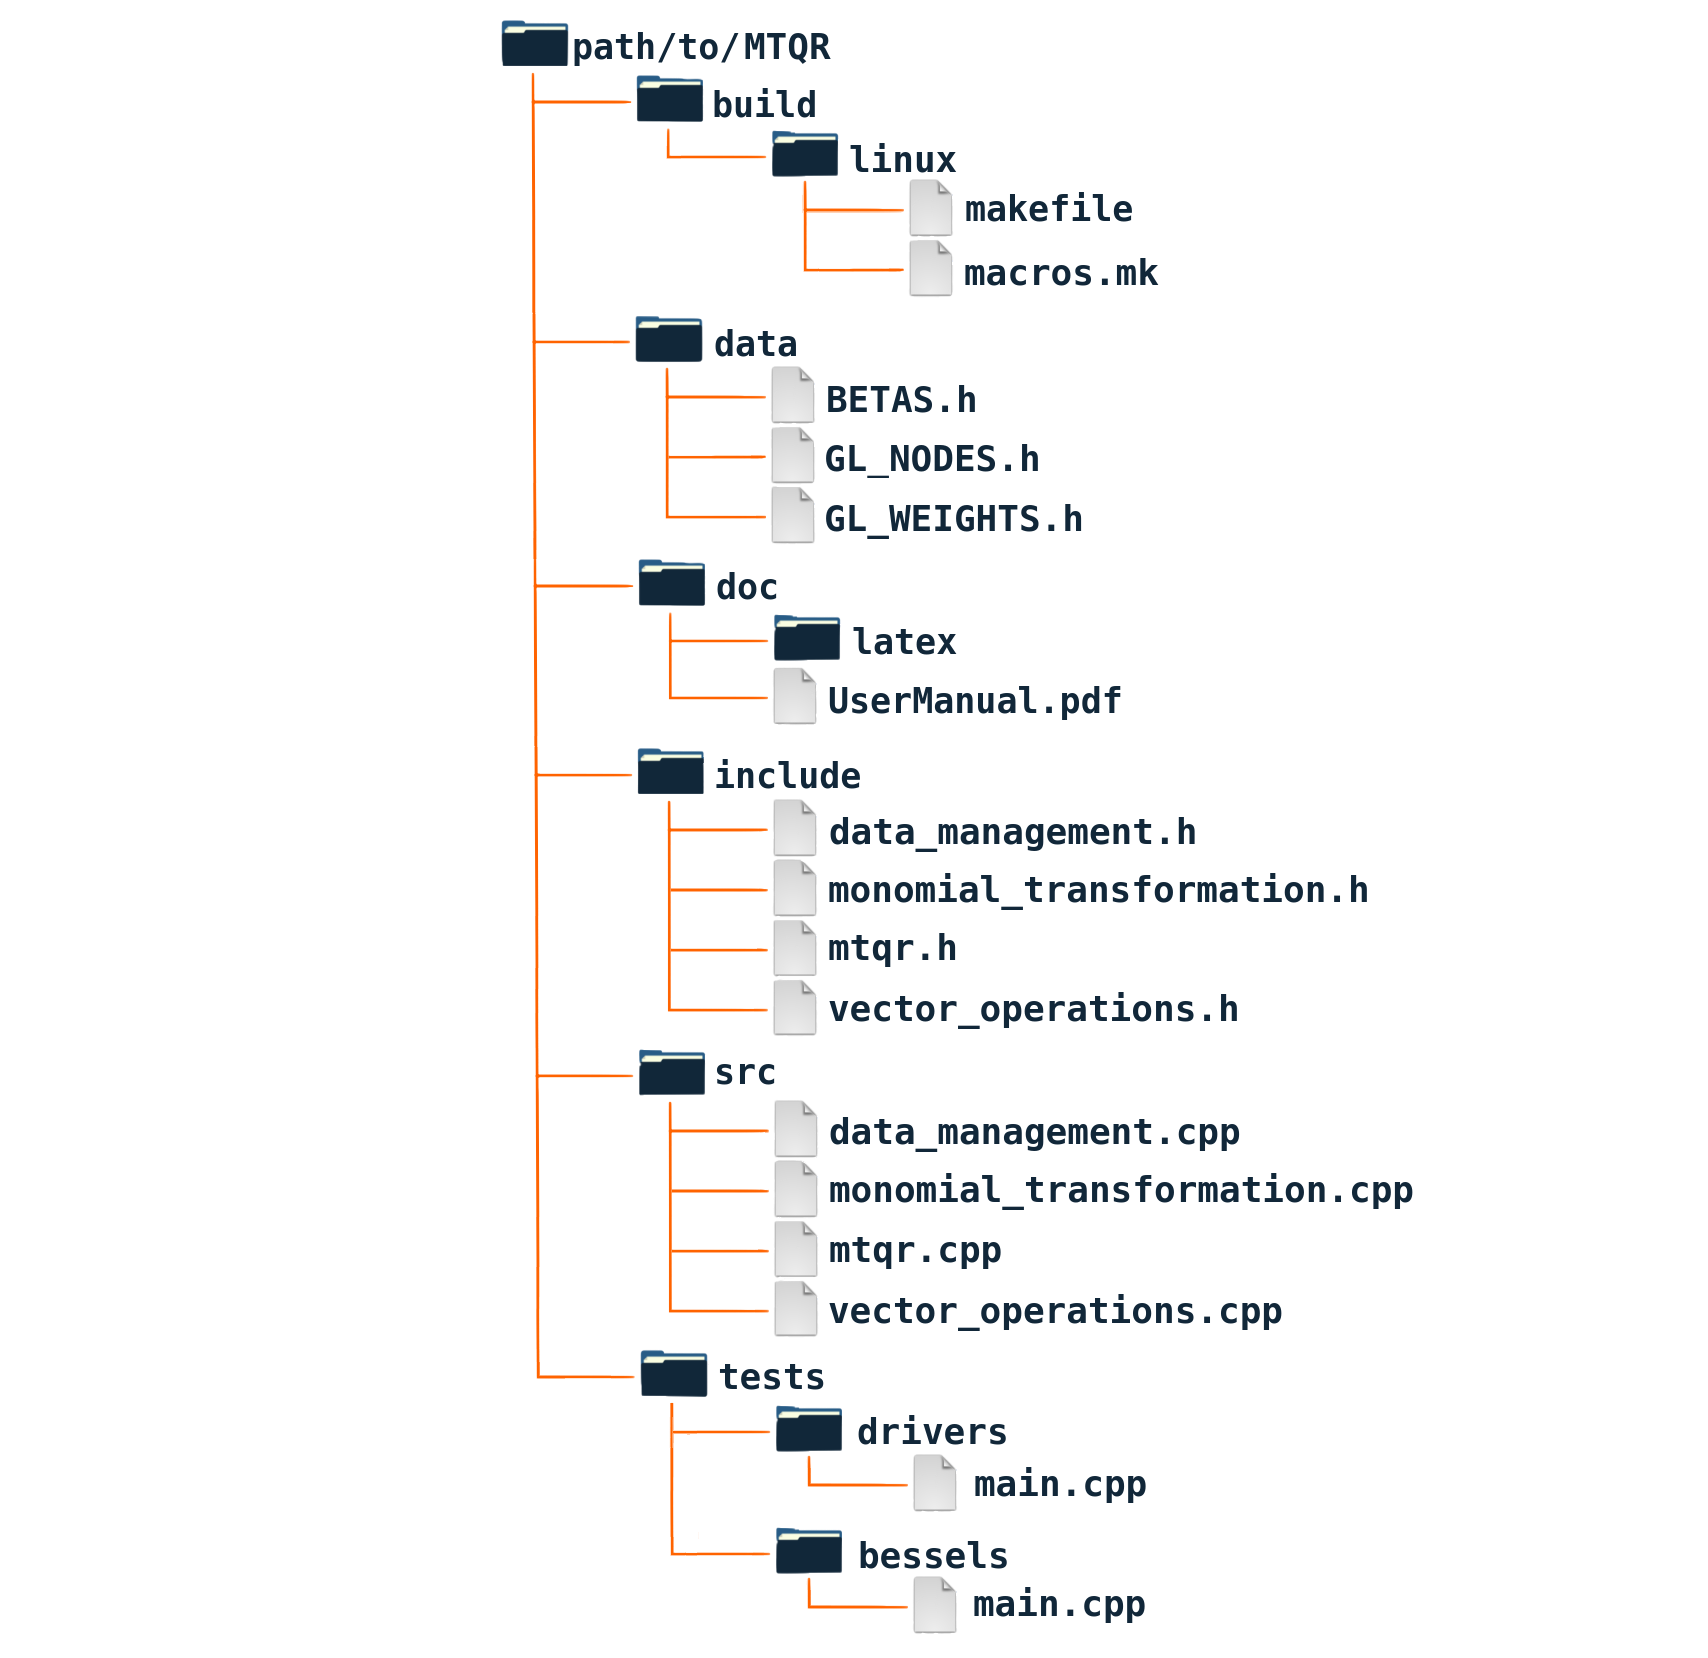
\includegraphics[keepaspectratio, width=.6\textwidth]{images/Fig2_1.png}
        \caption{The directory tree representing the structure and organisation of MTQR}
        \label{Fig2.1}
        \end{figure}
\end{center}

\noindent 
 Those header files are:
\begin{itemize}
    \item \colorbox{poliGrayBlue}{BETAS.h} collecting the values of $\beta_{\text{min}}(n)$ and $\beta_{\text{max}}(n)$ for each even value of $n\in[10,100]$;
    \item \colorbox{poliGrayBlue}{GL\_NODES.h} storing the G-L quadrature nodes in $(0,1)$ for each even value of $n\in[10,100]$;
    \item \colorbox{poliGrayBlue}{GL\_WEIGHTS.h} storing the weights of the G-L quadrature formula for each even value of $n\in[10,100]$.
\end{itemize}
The last two header files store the tabulated values of the original G-L nodes and weights both mapped in $(0,1)$ with 34 digits (only even-valued number of samples have been stored for the sake of simplicity). Their automatic computation is outside the scope of the library and already explored in details and implemented in other works \cite{Gautschi94,Hale13}. The folder \colorbox{poliGrayBlue}{\textbf{MTQR/build}} is used to collect the output files of the build setup instantiated by CMake and the sub-folder \colorbox{poliGrayBlue}{\textbf{MTQR/build/linux}} contains the aforementioned \colorbox{poliGrayBlue}{makefile} that Linux users can exploit as an alternative to CMake in order to build MTQR.

\section[Build process]{\changefont BUILD PROCESS}\sectionmark{BUILD PROCESS}\label{Sec2.3}

\noindent
MTQR is a quadrature tool that can be easily integrated in any user applications. As is the case for most C++ open-source software, once the (static) library is compiled succesfully, the user can choose to either create stand-alone applications (as exemplified by the scripts contained in the \colorbox{poliGrayBlue}{\textbf{MTQR/tests}} sub-directory) or use the primary module within a much larger codebase s.a. finite elements solvers and other implemented numerical methods. Regardless of the preferred choice, in order to use MTQR's features the user must not forget to link the desired application against the static library (following the build).

\subsection[Linux]{\changefont LINUX}\label{SubSec2.3.1}

In Linux the user can build MTQR by running the \colorbox{poliGrayBlue}{autoinstall} command. The additional flag \colorbox{poliGrayBlue}{all} can be appended by the user to also compile the testing applications in \colorbox{poliGrayBlue}{\textbf{MTQR/tests}} (see Section \ref{Sec2.4}) as shown below.

\begin{tcblisting}{enhanced,
                   arc=5mm,
                   title = \color{black}{\large \ttfamily Build using the shell script},
                   colbacktitle=bashGray,
                   colback=bashBlue,
                   listing only,
                   listing style=BashStyle}
user@machine: MTQR > ./autoinstall all
 *** INSTALLING MTQR ***

g++ -c ../../src/mtqr.cpp -o obj/mtqr.o -g -ansi -std=c++17  -I../../include  -I../../data
g++ -c ../../src/data_management.cpp -o obj/data_management.o -g -ansi -std=c++17  -I../../include  -I../../data
g++ -c ../../src/monomial_transformation.cpp -o obj/monomial_transformation.o -g -ansi -std=c++17  -I../../include  -I../../data
g++ -c ../../src/vector_operations.cpp -o obj/vector_operations.o -g -ansi -std=c++17  -I../../include  -I../../data
ar rcs ../libmtqr.a obj/mtqr.o obj/data_management.o obj/monomial_transformation.o obj/vector_operations.o
Compiling tests...
...done!
Cleaning object files...
...done!
 
 *** INSTALLATION COMPLETED ***

 user@machine: MTQR >
\end{tcblisting}
\vspace{0.25cm}

\noindent
Alternatively, the user can run \colorbox{poliGrayBlue}{cmake} from the library's root directory and, once completed, execute \colorbox{poliGrayBlue}{make} to create the static library and also compile and link all of the aforementioned testing applications into executables. Regardless of the procedure selected by the user, the static library \colorbox{poliGrayBlue}{libmtqr.a} will always be placed in \colorbox{poliGrayBlue}{\textbf{MTQR/build}} therefore the user shall either relocate such file in a directory included in the \colorbox{poliGrayBlue}{PATH} variable (e.g. \colorbox{poliGrayBlue}{\textbf{usr/lib}} or \colorbox{poliGrayBlue}{\textbf{usr/share}}) or specify the full path to \colorbox{poliGrayBlue}{libmtqr.a} to the linker.

\vspace{0.2cm}
\begin{tcblisting}{enhanced,
                   arc=5mm,
                   title = \color{black}{\large \ttfamily Build using CMake},
                   colbacktitle=bashGray,
                   colback=bashBlue,
                   listing only,
                   listing style=BashStyle}
user@machine: MTQR> cmake .
-- The CXX compiler identification is GNU 11.3.0
-- Detecting CXX compiler ABI info
-- Detecting CXX compiler ABI info - done
-- Check for working CXX compiler: /usr/bin/c++ - skipped
-- Detecting CXX compile features
-- Detecting CXX compile features - done
-- Found GSL: /usr/include (found version "2.7.1") 
-- Found Boost: /usr/lib/x86_64-linux-gnu/cmake/Boost-1.74.0/BoostConfig.cmake (found version "1.74.0")  
-- Configuring done
-- Generating done
-- Build files have been written to: /home/MTQR

user@machine: MTQR> make
[  5%] Building CXX object CMakeFiles/mtqr.dir/src/mtqr.cpp.o
[ 11%] Building CXX object CMakeFiles/mtqr.dir/src/data_management.cpp.o
[ 17%] Building CXX object CMakeFiles/mtqr.dir/src/monomial_transformation.cpp.o
[ 23%] Building CXX object CMakeFiles/mtqr.dir/src/vector_operations.cpp.o
[ 29%] Linking CXX static library build/libmtqr.a
[ 29%] Built target mtqr
[ 35%] Building CXX object CMakeFiles/drivers.dir/tests/drivers/main.cpp.o
[ 41%] Linking CXX executable build/drivers
[ 41%] Built target drivers
[ 47%] Building CXX object CMakeFiles/monomial.dir/tests/monomial/main.cpp.o
[ 52%] Linking CXX executable build/monomial
[ 52%] Built target monomial
[ 94%] Building CXX object CMakeFiles/bessel.dir/tests/bessel/main.cpp.o
[100%] Linking CXX executable build/bessel
[100%] Built target bessel

user@machine: MTQR>
\end{tcblisting}

\newpage

\subsection[Windows]{\changefont WINDOWS}\label{SubSec2.3.2}

We recommend using Microsoft Visual Studio as it automatically detects and runs CMake with the appropriate flags whenever a directory containing a \colorbox{poliGrayBlue}{CMakeLists.txt} is selected. Below is an example of the output from the terminal window when opening the library's root directory \colorbox{poliGrayBlue}{mtqr} in Visual Studio\footnote{By selecting \colorbox{poliGrayBlue}{open a local folder} immediately after starting Visual Studio.}.

\begin{tcblisting}{enhanced,
                   arc=5mm,
                   title = \color{black}{\large \ttfamily Build using Visual Studio},
                   colbacktitle=bashGray,
                   colback=black,
                   listing only,
                   listing style=PSStyle}
1> CMake generation started for configuration: 'x64-Debug'.
1> Found and using vcpkg toolchain file (C:/vcpkg/scripts/buildsystems/vcpkg.cmake).
1> Command line: "C:\WINDOWS\system32\cmd.exe" /c  ...
1> Working directory: C:\MTQR\out\build\x64-Debug
1> [CMake] -- The CXX compiler identification is MSVC 19.34.31937.0
1> [CMake] -- Detecting CXX compiler ABI info
1> [CMake] -- Detecting CXX compiler ABI info - done
1> [CMake] -- Check for working CXX compiler: C:/Program Files/Microsoft Visual Studio/2022/Community/VC/Tools/MSVC/14.34.31933/bin/Hostx64/x64/cl.exe - skipped
1> [CMake] -- Detecting CXX compile features
1> [CMake] -- Detecting CXX compile features - done
1> [CMake] -- Found GSL: C:/vcpkg/installed/x64-windows/include (found version "2.7.1") 
1> [CMake] -- Found Boost: C:/boost (found version "1.81.0")  
1> [CMake] -- Configuring done
1> [CMake] -- Generating done
1> [CMake] -- Build files have been written to: C:/MTQR/out/build/x64-Debug/build
1> Extracted CMake variables.
1> Extracted source files and headers.
1> Extracted code model.
1> Extracted toolchain configurations.
1> Extracted includes paths.
1> CMake generation finished.
\end{tcblisting}
\vspace{0.3cm}

\noindent
Once CMake terminates the procedure, the user can head to the \colorbox{poliGrayBlue}{Solution explorer} (most often located on the left or right panel of Visual Studio), click on the \colorbox{poliGrayBlue}{Switch between solutions and available views} button and double-click on \colorbox{poliGrayBlue}{CMake Targets View} and expand \colorbox{poliGrayBlue}{mtqr project}.
Among the list of all possible targets the user shall first compile the one named \colorbox{poliGrayBlue}{mtqr (static library)} by left-clicking on it and select \colorbox{poliGrayBlue}{Build} which, if successful, yields to the following output from the terminal.
\newline
Following the above the \colorbox{poliGrayBlue}{mtqr.lib} file will be available in \colorbox{poliGrayBlue}{\textbf{MTQR\textbackslash out\textbackslash build\textbackslash x64-Debug\textbackslash build}} sub-directory. At this point the user is ready to link any application to the static library or running the proposed test cases shipped with the library's source code.

\vspace{0.2cm}
\begin{tcblisting}{enhanced,
                   arc=5mm,
                   title = \color{black}{\large \ttfamily Compiling the static library target},
                   colbacktitle=bashGray,
                   colback=black,
                   listing only,
                   listing style=PSStyle}
>------ Build started: Project: CMakeLists, Configuration: Debug ------
  [1/5] Building CXX object CMakeFiles\mtqr.dir\src\mtqr.cpp.obj
C:\boost\boost\multiprecision\cpp_bin_float.hpp(2150): warning C4193: #pragma warning(pop): no matching '#pragma warning(push)'
  [2/5] Building CXX object CMakeFiles\mtqr.dir\src\vector_operations.cpp.obj
C:\boost\boost\multiprecision\cpp_bin_float.hpp(2150): warning C4193: #pragma warning(pop): no matching '#pragma warning(push)'
  [3/5] Building CXX object CMakeFiles\mtqr.dir\src\data_management.cpp.obj
C:\boost\boost\multiprecision\cpp_bin_float.hpp(2150): warning C4193: #pragma warning(pop): no matching '#pragma warning(push)'
  [4/5] Building CXX object CMakeFiles\mtqr.dir\src\monomial_transformation.cpp.obj
C:\boost\boost\multiprecision\cpp_bin_float.hpp(2150): warning C4193: #pragma warning(pop): no matching '#pragma warning(push)'
C:\MTQR\src\monomial_transformation.cpp(105): warning C4244: '=': conversion from 'double' to 'int', possible loss of data
  [5/5] Linking CXX static library mtqr.lib
\end{tcblisting}
\vspace{0.3cm}

\section[Testing the build]{\changefont TESTING THE BUILD}\sectionmark{TESTING THE BUILD}\label{Sec2.4}

\noindent
After the successful compilation of the library the user is ready to instantiate MTQR's primary module in any desired application. It is however a widespread good-practice to test the build of an installed library before proceeding with its usage and this principles becomes particularly truthful in the case of MTQR. For that purpose we prepared few test applications, located in the aforementioned \colorbox{poliGrayBlue}{\textbf{MTQR/tests}} which not only satisfy the sanity-check principle for the build but, in our opinion, also provide the user with an aid on how to use MTQR via its primary module and therefore ease its implementation in larger codebase. We remark that these tests have been successfully ran on all the platforms listed in Table \ref{table2.1}; given the compatibility with multiple architectures we will only refer to the results obtained and omit the specifications for the system on which they have been derived since they do not vary. Furthermore we reiterate that if the library has been built using CMake the executables of the test cases will be located in \colorbox{poliGrayBlue}{\textbf{MTQR/build}} on Linux systems (\colorbox{poliGrayBlue}{\textbf{MTQR/build/linux}} if compiled using \colorbox{poliGrayBlue}{autoinstall all}) and in \colorbox{poliGrayBlue}{\textbf{MTQR\textbackslash out\textbackslash build\textbackslash x64-Debug\textbackslash build}} on Windows (using Microsoft Visual Studio). For the sake of completeness we show how the \colorbox{poliGrayBlue}{drivers} test is built on Windows while we compile and execute the \colorbox{poliGrayBlue}{bessels} test on Linux.

\subsection[Drivers]{\changefont DRIVERS}\label{SubSec2.4.1}

In the \colorbox{poliGrayBlue}{\textbf{MTQR/tests/drivers}} sub-directory the \colorbox{poliGrayBlue}{main.cpp} file contains a very straight-forward yet powerful example of how an application can be built by the user with MTQR. It presents three tests cases where we want to integrate three functions that are very different among each others. The three polynomial functions are the following

\begin{equation*}
    \begin{split}
        p_1(x) & = 5x^{-\frac{\pi}{4}}-x^{-\frac{1}{2}}+1+10x^{2}+ex^{e+\frac{1}{4}}\,, \\
        p_2(x) & = x^{-\frac{e}{3}}\,, \\
        p_3(x) & = x^{17} + x^{35}\,,
    \end{split}
\end{equation*}

\noindent
and, with the exception of $p_3(x)$, all have a singularity in $x=0$ (MTQR defaults the integration interval to be $(0,1)$). Using Visual Studio the workflow would be first to compile the executable associated to the present test case, which is accomplished by repeating the exact same steps outlined in Sub-Section \ref{SubSec2.3.2} except now they are done for the target \colorbox{poliGrayBlue}{drivers (executable)} listed in the \colorbox{poliGrayBlue}{Solution explorer} alongside the other executable targets.

\vspace{0.2cm}
\begin{tcblisting}{enhanced,
                   arc=5mm,
                   title = \color{black}{\large \ttfamily Compiling the drivers test case},
                   colbacktitle=bashGray,
                   colback=black,
                   listing only,
                   listing style=PSStyle}
[1/2] Building CXX object CMakeFiles\drivers.dir\tests\drivers\main.cpp.obj
C:\boost\boost\multiprecision\cpp_bin_float.hpp(2150): warning C4193: #pragma warning(pop): no matching '#pragma warning(push)'
[2/2] Linking CXX executable drivers.exe
\end{tcblisting}
\vspace{0.3cm}

\noindent
Once compiled, the executable can be run within Visual Studio itself by simply opening the integrated PowerShell terminal, navigating to \colorbox{poliGrayBlue}{\textbf{MTQR\textbackslash out\textbackslash build\textbackslash x64-Debug}} and running the \colorbox{poliGrayBlue}{drivers.exe} file. As evidenced below, the resulting application integrates each polynomial using the monomial transformation quadrature rule provided by MTQR through the primary module. We remark that, although no difference in numerical results occurs, the following report solely concerns the loud mode of execution. A list of information regarding the monomial transformation itself is displayed on the terminal whereas the results of interest (i.e. the new processed quadrature together with the related numerical integration) \color{black} are exported in files located in the appropriate output directory. 
\newline
The results of the quadrature and the new nodes and weights are then exported in three separate files called \colorbox{poliGrayBlue}{Results.txt}, \colorbox{poliGrayBlue}{Nodes.txt} and \colorbox{poliGrayBlue}{Weights.txt} all located in a \colorbox{poliGrayBlue}{\textbf{output}} directory created automatically at runtime in the same path of the user’s executable. To run the second and third benchmark the user needs to press \colorbox{poliGrayBlue}{ENTER} on whatever terminal the process is being paused on. Note that, since we are implementing three benchmark polynomials in a single source file, such pause is necessary during the execution in order to capture the new processed quadrature together with the associated numerical integration as the files in the output directory are overwritten at each execution.

\newpage
\begin{tcblisting}{enhanced,
                   arc=5mm,
                   title = \color{black}{\large \ttfamily Executing the driver test case: p\_1(x)},
                   colbacktitle=bashGray,
                   colback=black,
                   listing only,
                   listing style=PSStyle}
PS C:\MTQR> cd .\out\build\x64-Debug\
PS C:\MTQR\out\build\x64-Debug> .\drivers.exe

    |*************************************************|
    |                 ** MTQR **                      |
    |  ** MONOMIAL TRANSFORMATION QUADRATURE RULE **  |
    |*************************************************|


 Input polynomial p(x) =  +2.71828183*x^(2.96828183) +5*x^(-0.785398163) -1*x^(-0.5) +x^(0)  +10*x^(2)

 ** Accepted sequence of exponents **
    {2.96828183, -0.785398163, -0.5, 0, 2}
 ** Lambda_min = -0.785398163, Lambda_max = 2.96828183 **
 **************************************************
 ** N_min = 32
 ** Beta_min = 4.37782519, Beta_max = 127.894326 **
 ** Transformation order = 28.7703455 **
 **************************************************
 ** Using double f.p. format for nodes and weights **
 ** I(p(x))   = 26.317297376488324 **
 ** I_n(p(x)) = 26.317297376488324  [with parameters in float128 precision] **
 ** E_n(p(x)) = 1.3889468142066847e-17  [with parameters in float128 precision] **
 ** I_n(p(x)) = 26.317297376488324  [with parameters in double precision] **
 ** E_n(p(x)) = 5.4523153678583708e-18 [with parameters in double precision] **
\end{tcblisting}
\vspace{0.3cm}

\noindent
The correct execution of all three benchmarks will then close the application. The user should check that each benchmark is executed without problems and the results are correctly generated (see Section \ref{Sec3.2}). As for the quality of the results obtained for those tests, an in-depth analysis, coupled with the fast execution of the program, shows the advantages provided by MTQR over classical G-L and other generalised quadrature rules. The first polynomial $p_1(x)$ is a model proposed in equation (73) of \cite{Lombardi09}, \textsl{Section 5.1, Example 1}, and it represents a generalised polynomial integrand that might model cumbersome integrand function in numerical methods for differential and integral equations featuring singular modelling, on which MTQR is indeed considered an helpful, effective and precise tool for integration. The proposed generalised polynomial $p_1(x)$ features a singularity at $x=0$ in the interval $(0,1)$ and all but two of its monomial terms have non-integer degree. The numerical approximation of the integral at double precision is achieved with $n=32$ nodes using a monomial transformation applied to the classical G-L quadrature with $n$ nodes in $(0,1)$. The Table \ref{table2.2} below shows what was graphically reported in Figure \ref{Fig1.2} i.e. the ad-hoc suited and more efficient distribution of the samples obtained by the monomial transformation as opposed to the ones of the classical G-L quadrature rule. While in fact we know that the $n=32$ nodes of the classical G-L quadrature rule are distributed symmetrically in $(0,1)$ with an equal abundance of those at both bounds of the integration interval, our proposed quadrature scheme, based on the monomial transformation, concentrates the samples close to the lower bound $x=0$, squashing the vast majority of them ($26$ out of the total $32$) inside the sub-interval $(0,0.1)$ thereby better capturing the singular behaviour of $p_1(x)$. Notice how, while instantiating the primary module for $p_1(x)$, we generate a precision quadrature for all generalised polynomials with sets of $\lambda \in [\lambda_{\text{min}},\lambda_{\text{max}}]=[-\pi/4,e+1/4]$. The second benchmark polynomial is proposed with the scope of introducing the user to a core functionality of MTQR that requires further input on the CLI. Indeed, $p_2(x)$ is a monomial of non-integer degree and its numerical integration requires careful manipulation. During the modelling process of larger applications, especially when dealing with finite elements constructed over meshed domains with singular spatial geometry behaviour \cite{Graglia04,Graglia08} it is often necessary to integrate singular generalised polynomial basis functions together with high-order regular polynomial basis functions. 
\newline
MTQR allows to integrate such integrals identifying the degree of the monomial as $\lambda_{\text{min}}$ and the maximum degree  $\lambda_{\text{max}}$ of the all set of combined polynomial functions. For this reason, in this test, we add a monomial with $\lambda_{\text{max}}$ degree and unitary coefficient to $p_2(x)$. Once constructed the final polynomial we apply the proposed algorithm to process the optimised nodes and weights. In this case we set $r=r_{\text{min}}$ as in $(\ref{eq1.17})$ and then we compute $\lambda_{\text{max}} = \frac{\beta_{\text{max}(n)} -r+1}{r}$ (see Equation (52) in \cite{Lombardi09}). This procedure is a specialized execution of MTQR.
\newline
In test case 2, the integration is enabled using a caveat prompted on the terminal and it consists in choosing one path between two mutually exclusive options that the user must exercise in order to continue with the application.

\newpage
\vspace{0.2cm}
\begin{table}[H]
\centering
\begin{tabular}{|c||c|c|}
\hline
\multicolumn{3}{|c|}{\textbf{Nodes and weights of the proposed quadrature for $p_1(x)$ }} \\
\hline
$j\in\mathbb{N}$ & $x_j\in(0,1)$ & $w_j\in\mathbb{R}^+$ \\
\hline
1   &  4.0256721894941735e-83  &  2.9709584266857193e-81  \\
2   &  2.2116841854653406e-62  &  7.1971053989801097e-61  \\
3   &  3.4370358897566318e-51  &  7.1255611223692978e-50  \\
4   &  1.6010758830624544e-43  &  2.4253789034229506e-42  \\
5   &  1.0479208102676717e-37  &  1.2456363438765983e-36  \\
6   &  4.8718071131884711e-33  &  4.7453741025535338e-32  \\
7   &  3.7119919463646725e-29  &  3.0494845207591382e-28  \\
8   &  7.5510919371932376e-26  &  5.3393428605147779e-25  \\
9   &  5.58947068987428e-23    &  3.4526789629984772e-22  \\
10  &  1.8549840400142102e-20  &  1.0121884313459638e-19  \\
11  &  3.1981531227726135e-18  &  1.5545919457374846e-17  \\
12  &  3.1905126409913618e-16  &  1.3904418738462426e-15  \\
13  &  1.9974633805093215e-14  &  7.8421013950383668e-14  \\
14  &  8.3548669580378659e-13  &  2.9653252968844048e-12  \\
15  &  2.4525558094710645e-11  &  7.8879379262599627e-11  \\
16  &  5.2553535644885825e-10  &  1.5337625816699302e-09  \\
17  &  8.4865615532959245e-09  &  2.2485149221054993e-08  \\
18  &  1.0601166175497224e-07  &  2.5487504629916981e-07  \\
19  &  1.0467771915132323e-06  &  2.2805293469267595e-06  \\
20  &  8.3187859060800558e-06  &  1.6383778757563812e-05  \\
21  &  5.4017656350748472e-05  &  9.583886949817516e-05   \\
22  &  0.00029027719974030597  &  0.00046172220499588948  \\
23  &  0.0013048618829373392   &  0.0018488842315729846   \\
24  &  0.0049515587664587246   &  0.0061972140073356637   \\
25  &  0.01598386920155067     &  0.017474549464975012    \\
26  &  0.044176504650425052    &  0.041563995305652503    \\
27  &  0.10510275956828145     &  0.083385319613667491    \\
28  &  0.21621415218381346     &  0.14051580648196024     \\
29  &  0.38598199665949656     &  0.19670495174814193     \\
30  &  0.59964365548997856     &  0.22295968412650397     \\
31  &  0.81242716007987004     &  0.1915755472071223      \\
32  &  0.96137880664253184     &  0.097197543454586643    \\
\hline
\end{tabular}
  \caption{Nodes and weights obtained by a monomial transformation of order $r=28.77$ applied to the G-L quadrature integrating $p_1(x)$ in $(0,1)$ at double precision with $n=32$ samples.}
  \label{table2.2}
\end{table}

\vspace{0.2cm}
\begin{tcblisting}{enhanced,
                   arc=5mm,
                   title = \color{black}{\large \ttfamily Executing the driver test case: p\_2(x)},
                   colbacktitle=bashGray,
                   colback=black,
                   listing only,
                   listing style=PSStyle}
    |*************************************************|
    |                 ** MTQR **                      |
    |  ** MONOMIAL TRANSFORMATION QUADRATURE RULE **  |
    |*************************************************|

 Input polynomial p(x) =  +x^(-0.906093943) 

 ** WARNING ** Your input is a monomial of non-integer degree.
               MTQR needs a binomial for double-precision quadrature.
               How do you proceed? ['nodes' for n_min ~ 'lambda' for lambda_max]
               Input: 
\end{tcblisting}

\noindent
One of those is the choice of specifying the maximum number $n$ for the quadrature rule, in which case the library  automatically compute $\lambda_{\text{max}}$ and integrate $\tilde{p_2}(x) = x^{-\frac{e}{3}} + x^{\lambda_\text{max}}$ accordingly. The second path allows instead to specify $\lambda_{\text{max}}$ directly and let MTQR carry out the integration. It is easy to see that the second case reduces to a \textsl{"standard"} polynomial input, as far as the library is concerned. The user should therefore type \colorbox{poliGrayBlue}{nodes} on the CLI and press \colorbox{poliGrayBlue}{ENTER}; we are now prompted to select any value of $n\in[10,100]$; user should type, for example, $64$ and press \colorbox{poliGrayBlue}{ENTER} again. 

\vspace{0.2cm}
\begin{tcblisting}{enhanced,
                   arc=5mm,
                   title = \color{black}{\large \ttfamily Building and executing the test driver: p\_2(x)},
                   colbacktitle=bashGray,
                   colback=black,
                   listing only,
                   listing style=PSStyle}
Please specify the desired number of quadrature nodes (number must be even): 64
 **************************************************
 ** N_min = 64
 ** Beta_min = 3.25021668, Beta_max = 511.19448 **
 ** Accepted sequence of exponents ** 
    {-0.906093943, 10.3166381}
 ** Lambda_min = -0.906093943, Lambda_max = 10.3166381 **
 **************************************************
 ** N_min = 64
 ** Beta_min = 3.25021668, Beta_max = 511.19448 **
 ** Transformation order = 45.2603038 **
 **************************************************
 ** Using double f.p. format for nodes and weights **
 ** I(p(x))   = 10.737305800857456 **
 ** I_n(p(x)) = 10.737305800857441     [with parameters in float128 precision] **
 ** E_n(p(x)) = 1.424785764850455e-15  [with parameters in float128 precision] **
 ** I_n(p(x)) = 10.737305800857441     [with parameters in double precision] **
 ** E_n(p(x)) = 1.4344708669352776e-15 [with parameters in double precision] **

 ** MTQR HAS TERMINATED **
\end{tcblisting}
\vspace{0.3cm}

\begin{table}[H]
\hspace{-0.8cm}
\begin{tabular}{|c||c|c||c||c|c|}
\hline
\multicolumn{6}{|c|}{\textbf{Nodes and weights of the proposed quadrature for $p_2(x)$}} \\
\hline
$j\in\mathbb{N}$ & $x_j\in(0,1)$ & $w_j\in\mathbb{R}^+$ & $j\in\mathbb{N}$ & $x_j\in(0,1)$ & $w_j\in\mathbb{R}^+$ \\
\hline
1   & 2.7630147554775799e-157   & 3.2089404684705014e-155  & 33  & 7.0500634584281311e-14 & 1.5167370865604578e-13 \\
2   & 1.2504818169246583e-124   & 6.4130575288015817e-123  & 34  & 5.7559583188242479e-13 & 1.1793837946815465e-12 \\
3   & 5.6814585252048909e-107   & 1.8611939310882479e-105  & 35  & 4.2517694749483687e-12 & 8.2956748948158666e-12 \\
4   & 7.80153953804910668e-95   & 1.8746032945680622e-93   & 36  & 2.8538360103496875e-11 & 5.3006402608938980e-11 \\
5   & 1.37705792986285616e-85   & 2.6096113660080927e-84   & 37  & 1.7474698043212560e-10 & 3.0884893242340361e-10 \\
6   & 3.99955200879667989e-78   & 6.2503681667652076e-77   & 38  & 9.7966474232194539e-10 & 1.6467041924026613e-09 \\
7   & 7.12412148203568704e-72   & 9.4622687681839969e-71   & 39  & 5.0450425037572576e-09 & 8.0595541550951593e-09 \\
8   & 1.67758621116242340e-66   & 1.9352874634013771e-65   & 40  & 2.3937780380919019e-08 & 3.6314704984080236e-08 \\
9   & 8.50394804246417862e-62   & 8.6610446966327004e-61   & 41  & 1.0493924006829552e-07 & 1.5103117353143750e-07 \\
10  & 1.28937420430520282e-57   & 1.17417554134314e-56     & 42  & 4.2611947777521824e-07 & 5.8115902014625234e-07 \\
11  & 7.37695543314284930e-54   & 6.0678528535818764e-53   & 43  & 1.6064924620227659e-06 & 2.0734907170162103e-06 \\
12  & 1.88823854215581744e-50   & 1.4144870181471483e-49   & 44  & 5.6352337753679891e-06 & 6.8727595063813297e-06 \\
13  & 2.45874041791221323e-47   & 1.6888846224093984e-46   & 45  & 1.8428406102394049e-05 & 2.1200152242057246e-05 \\
14  & 1.79879095499131601e-44   & 1.1394463566176748e-43   & 46  & 5.6285102084355121e-05 & 6.0953635295967037e-05 \\
15  & 7.99644755427870559e-42   & 4.6939290576395100e-41   & 47  & 0.000160824501490444   & 0.00016357104996692    \\
16  & 2.30031834550869425e-39   & 1.256455692921632e-38    & 48  & 0.000430554366218858   & 0.000410178545783102   \\
17  & 4.50736224431423266e-37   & 2.2990244539015347e-36   & 49  & 0.001081507980701627   & 0.00096212522184789    \\
18  & 6.27605017641916653e-35   & 2.9984883056622040e-34   & 50  & 0.002552202028188329   & 0.002112665166000562   \\
19  & 6.43329661193267433e-33   & 2.8866958399889620e-32   & 51  & 0.005664918590851289   & 0.004345383033450631   \\
20  & 5.00167986643949820e-31   & 2.1127162036193374e-30   & 52  & 0.011839418057758923   & 0.008374932123081819   \\
21  & 3.02522544694279073e-29   & 1.2053618210763572e-28   & 53  & 0.023321020012667499   & 0.015126268661501289   \\
22  & 1.45485132139284000e-27   & 5.4774213217611214e-27   & 54  & 0.043333892814950261   & 0.025596514741963807   \\
23  & 5.66857779784746315e-26   & 2.0197293557945103e-25   & 55  & 0.076017823001042698   & 0.040555711474099192   \\
24  & 1.81901613177956244e-24   & 6.1417478949789698e-24   & 56  & 0.1259851142914331     & 0.060094184332119245   \\
25  & 4.87674410785629622e-23   & 1.5621281667244454e-22   & 57  & 0.197384568387222875   & 0.083114399815460055   \\
26  & 1.10619188116815056e-21   & 3.3648881412038240e-21   & 58  & 0.292508401834271963   & 0.106964653637029898   \\
27  & 2.14674169704207817e-20   & 6.2062442929374053e-20   & 59  & 0.410207778274644215   & 0.127463313674079491   \\
28  & 3.59979724510255679e-19   & 9.8975903331295861e-19   & 60  & 0.544613347654060773   & 0.139504287218888873   \\
29  & 5.26211017870698955e-18   & 1.3767307083491291e-17   & 61  & 0.68476273369408191    & 0.138243738177407818   \\
30  & 6.75862034692174972e-17   & 1.68331269687316e-16     & 62  & 0.815603424165963892   & 0.120596149243306058   \\
31  & 7.68166812405570700e-16   & 1.8218265936883635e-15   & 63  & 0.920443566774952144   & 0.086540144565319482   \\
32  & 7.77553771704852579e-15   & 1.756314510825820e-14    & 64  & 0.984393322175774548   & 0.039739900698273792   \\
\hline
\end{tabular}
  \caption{Nodes and weights obtained by a monomial transformation of order $r=45.26$ applied to $p_2(x)$.}
  \label{table2.3}
\end{table}

\noindent
On the contrary typing \colorbox{poliGrayBlue}{lambda} causes the application to resort to its original workflow with the additional intermediate step of requiring the input value of $\lambda_{\text{max}}$. We remark that any miss-typed or empty input results in MTQR to throw an error message and exit the program. After the specified selection, MTQR computes automatically a value of $\lambda_{\text{max}} = 10.3166381$ for $p_2(x)$ and the resulting quadrature barely retains the machine-epsilon double precision for the relative error of the numerical integration. Here, the library is stressed more as it can be evinced by the substantially greater value of the transformation order $(r=45.2603038)$ w.r.t. the previous instance in $p_1(x)$. Furthermore we highlight how the relative error obtained with \colorbox{poliGrayBlue}{float128} monomial transformation quadrature rule's parameters is not substantially better than the one derive with the same nodes and weights optimised in double f.p. format\footnote{We remark that the computationally expensive \colorbox{poliGrayBlue}{float128} format has been implemented to secure precision in the execution of the algorithm, even if we did not experience any improvement with respect to double format in our tests.\vspace{-2ex}}.

\vspace{0.1cm}
\begin{tcblisting}{enhanced,
                   arc=5mm,
                   title = \color{black}{\large \ttfamily Executing the driver test case: p\_3(x)},
                   colbacktitle=bashGray,
                   colback=black,
                   listing only,
                   listing style=PSStyle}
    |*************************************************|
    |                 ** MTQR **                      |
    |  ** MONOMIAL TRANSFORMATION QUADRATURE RULE **  |
    |*************************************************|
    
Input polynomial p(x) =  +x^(17)  +x^(35) 

 ** Accepted sequence of exponents ** 
    {17, 35}
 ** Lambda_min = 17, Lambda_max = 35 **
 **************************************************
 ** N_min = 12
 ** Beta_min = 8.54130275, Beta_max = 23.2002133 **
 ** Transformation order = 0.601150262 **
 **************************************************
 ** Using double f.p. format for nodes and weights **
 ** I(p(x))   = 0.083333333333333333 **
 ** I_n(p(x)) = 0.083333333333333326    [with parameters in float128 precision] **
 ** E_n(p(x)) = 8.8727918916220005e-17  [with parameters in float128 precision] **
 ** I_n(p(x)) = 0.083333333333333323    [with parameters in double precision] **
 ** E_n(p(x)) = 1.1803389750004119e-16  [with parameters in double precision] **

 ** MTQR HAS TERMINATED **

PS C:\MTQR\out\build\x64-Debug> 
\end{tcblisting}

\noindent 
Finally, with the last benchmark a classical polynomial of high integer-degree is integrated. According described in Sub-Section \ref{SubSec1.2.2}, G-L requires $n=\frac{\lambda_{max}+1}{2}=18$ samples to achieve double precise integration for classical polynomials up to degree $35$. We immediately realise that MTQR  outperforms the classical G-L quadrature rule for a fixed machine accuracy as only $n=12$ samples are needed. Since $p_3(x)$ does not have a singularity at $x=0$ and therefore the nodes in MTQR are not clustered on $x=0$. Instead the transformation forces the performance of the quadrature to effectively integrate all generalised polynomials with $\lambda\in[17,35]$ at machine-epsilon precision.

\begin{table}[H]
\centering
\begin{tabular}{|c||c|c|}
\hline
\multicolumn{3}{|c|}{\textbf{Nodes and weights of the proposed quadrature for $p_3(x)$}} \\
\hline
$j\in\mathbb{N}$ & $x_j\in(0,1)$ & $w_j\in\mathbb{R}^+$ \\
\hline
1   &  0.0597707229696358   &  0.0919264663553836  \\
2   &  0.1610307309568925   &  0.1079664407846363  \\
3   &  0.2725515941208583   &  0.1139863183561349  \\
4   &  0.3872246099856674   &  0.1145999654489373  \\
5   &  0.5003873977306973   &  0.1111039615531504  \\
6   &  0.6082809536783961   &  0.1041479683059256  \\
7   &  0.7076854327640707   &  0.0941968566214454  \\
8   &  0.7958143666363263   &  0.0816648573999376  \\
9   &  0.8702918448156044   &  0.0669634924046180  \\
10  &  0.9291601555462656   &  0.0505192348221430  \\
11  &  0.9708981507831240   &  0.0327793590987762  \\
12  &  0.9944473508291223   &  0.0142322139984140  \\
\hline
\end{tabular}
  \caption{Nodes and weights obtained by a monomial transformation of order $r=0.6011$ applied to $p_3(x)$ in (0,1).}
  \label{table2.4}
\end{table}

\noindent
With these results we would like to direct the user's attention on the possibility of using MTQR even for specific standard/classical polynomials of integer degree as its processed quadrature samples lead to fewer evaluations in the quadrature rule (especially with higher-degrees) and thus more efficient and less expensive code to run.

\subsection[Bessel]{\changefont BESSEL}\label{SubSec2.4.2}
We now address the building process for applications using MTQR on Linux by compiling and executing the \colorbox{poliGrayBlue}{\textbf{MTQR/tests/bessels}} numerical example that integrates Bessel functions of fractional order \cite{Abramowitz} which are expressed with a series expansion of the form

\begin{equation*}
    J_{\nu}(x) = \bigg(\frac{1}{2}x\bigg)^{\nu}\sum_{m=0}^{+\infty}\bigg(\frac{(-\frac{1}{4}x^2)^{m}}{m!\,\Gamma(\nu+m+1)}\bigg)\,,\quad\nu>-1
\end{equation*}

\noindent
where $\Gamma(z)=\int_0^{+\infty}x^{z-1}e^{-x}dx$ is Euler's gamma function. Similar results can also be achieved while using different representation of Bessel functions. As with the previous test, the standalone \colorbox{poliGrayBlue}{main.cpp} script treats three separate integrands\footnote{Evaluated using GSL's \colorbox{poliGrayBlue}{gsl$\_$sf$\_$bessel$\_$Jnu} built-in function}, specifically

\begin{equation*}
    \begin{split}
        b_1(x) & = J_{-\frac{1}{2}}(x)\,,\quad\bigg[\lambda_{\text{min}}=-\frac{1}{2},\, \lambda_{\text{max}}=\frac{15}{2}\bigg]\,, \\
        b_2(x) & = J_{-\frac{1}{2}}(x) + J_{\frac{1}{3}}(x)\,,\quad\bigg[\lambda_{\text{min}}=-\frac{1}{2},\, \lambda_{\text{max}}=\frac{25}{3}\bigg]\,, \\
        b_3(x) & = J_{-\frac{1}{2}}(x)\,J_{1}(x)\,,\quad\bigg[\lambda_{\text{min}}=\frac{1}{2},\, \lambda_{\text{max}}=\frac{33}{2}\bigg]\,,
    \end{split}
\end{equation*}

\noindent
all truncated up to the first $m=5$ terms. As explained in Sub-Section \ref{SubSec2.3.1} compiling the library using the built-in command \colorbox{poliGrayBlue}{autoinstall all} will make the executable of both tests readily available. Therefore, from the \colorbox{poliGrayBlue}{\textbf{MTQR/build/linux}} sub-directory we can easily launch the \colorbox{poliGrayBlue}{bessels} executable

\vspace{0.2cm}
\begin{tcblisting}{enhanced,
                   arc=5mm,
                   title = \color{black}{\large \ttfamily Executing the bessels test case: b\_1(x)},
                   colbacktitle=bashGray,
                   colback=bashBlue,
                   listing only,
                   listing style=BashStyle}
user@machine: MTQR/build/linux > ./bessels 
Iteration n. 1:  In=1.4434118505832414, En=1.3842419943602952e-09   (n. samples=18)
Iteration n. 2:  In=1.4434118485851772, En=2.2767307585229809e-14   (n. samples=24)
Iteration n. 3:  In=1.4434118485852097, En=3.0766631871932174e-16   (n. samples=28)
Iteration n. 4:  In=1.4434118485852099, En=1.5383315935966087e-16   (n. samples=32)

\end{tcblisting}
\vspace{0.3cm}

\noindent
In this (and also the other examples of the \colorbox{poliGrayBlue}{bessels} tests) we perform $4$ iterations in which the integrand is truncated with increasingly more terms in the series expansion; so for the first iteration we only consider the first $m=2$ terms of the series, at the second iteration we consider a slightly more accurate truncation with $m=3$ terms and so on until we reach the $m=5$ terms truncation at the fourth and last iteraton. As printed on the terminal, it is evident that, while using MTQR, only $m=4$ terms are necessary to achieve double machine precision in terms of relative error for the integration of $b_1(x)$ using $n=28$ samples, i.e. we build an MTQR rule for $\lambda\in (-1/2, 15/2)$. Notice that in this test we are instantiating MTQR's \textit{silent} mode which, as addressed later in Section \ref{Sec3.2.bis}, exports the optimised quadrature samples at runtime while also parsing them (in double f.p. format) in a single \colorbox{poliGrayBlue}{outputs.txt}. Such nodes and weights are reported in Table \ref{table2.5} for the specific case of $b_1(x)$. Pressing \colorbox{poliGrayBlue}{ENTER} on the terminal will cause the program to progress to the integration of $b_2(x)$. 

\vspace{0.2cm}
\begin{tcblisting}{enhanced,
                   arc=5mm,
                   title = \color{black}{\large \ttfamily Executing the bessels test case: b\_2(x)},
                   colbacktitle=bashGray,
                   colback=bashBlue,
                   listing only,
                   listing style=BashStyle}

Iteration n. 1:  In=2.0616765364427128, En= 1.5093001397369456e-11   (n. samples=20)
Iteration n. 2:  In=2.0616765364115950, En= 4.3080396173398953e-16   (n. samples=26)
Iteration n. 3:  In=2.0616765364115954, En= 2.1540198086699477e-16   (n. samples=30)
Iteration n. 4:  In=2.0616765364115959, En= 0   (n. samples=32)

\end{tcblisting}
\vspace{0.3cm}

\noindent
whose results are reported in Table \ref{table2.6}; in this case we achieve double precision already at the second iteration with $m=3$ terms approximated using $n=26$ samples in the quadrature formula. Pressing \colorbox{poliGrayBlue}{ENTER} once more the final generalised polynomial $b_3(x)$ will be integrated

\vspace{0.2cm}
\begin{tcblisting}{enhanced,
                   arc=5mm,
                   title = \color{black}{\large \ttfamily Executing the bessels test case: b\_3(x)},
                   colbacktitle=bashGray,
                   colback=bashBlue,
                   listing only,
                   listing style=BashStyle}

Iteration n. 1:  In=0.20217936665914402, En= 4.6538577547142047e-14   (n. samples=16)
Iteration n. 2:  In=0.20217936665913455, En= 2.7456387933417138e-16   (n. samples=20)
Iteration n. 3:  In=0.20217936665913452, En= 4.1184581900125707e-16   (n. samples=24)
Iteration n. 4:  In=0.20217936665913455, En= 2.7456387933417138e-16   (n. samples=26)

\end{tcblisting}
\vspace{0.3cm}

\noindent
which can be checked against Table \ref{table2.7}. Once again we reach double precision at the second iteration $(m=3)$ with $n=20$ samples. 

\vspace{0.2cm}
\begin{table}[H]
\centering
\begin{tabular}{|c||c|c|}
\hline
\multicolumn{3}{|c|}{\textbf{Nodes and weights of the proposed quadrature for $b_1(x)$ }} \\
\hline
$j\in\mathbb{N}$ & $x_j\in(0,1)$ & $w_j\in\mathbb{R}^+$ \\
\hline
1   &  2.4886199426064151e-37  &  8.4962373994555118e-36  \\
2   &  9.7331836637461709e-28  &  1.4643479611244592e-26  \\
3   &  1.4457358100950039e-22  &  1.3842522302572618e-21  \\
4   &  5.0016005668192019e-19  &  3.4937303742677519e-18  \\
5   &  2.3898895696221016e-16  &  1.3072205683995924e-15  \\
6   &  3.3379176999637574e-14  &  1.4921737796227685e-13  \\
7   &  2.0061814162880028e-12  &  7.5396111250023958e-12  \\
8   &  6.5024461302093438e-11  &  2.0952062117980374e-10  \\
9   &  1.3114937396033565e-09  &  3.6747077855002399e-09  \\
10  &  1.8127051625051056e-08  &  4.4623882566268086e-08  \\
11  &  1.8378134371548134e-07  &  4.0048601618886300e-07  \\
12  &  1.4364127550661674e-06  &  2.7856943512053638e-06  \\
13  &  8.9845181012671335e-06  &  1.5562277176261812e-05  \\
14  &  4.6284863157369641e-05  &  7.1752397117410841e-05  \\
15  &  0.00020086526821504015  &  0.00027887690430810123  \\
16  &  0.00074763338591703199  &  0.00092899238516954601  \\
17  &  0.00242144448149024960  &  0.00268729403322269480  \\
18  &  0.00690521329493283800  &  0.00681984845919765200  \\
19  &  0.01750612415771758700  &  0.01530440169550289400  \\
20  &  0.03977115705124230300  &  0.03054591754739828500  \\
21  &  0.08150130998495218300  &  0.05442760391046814300  \\
22  &  0.15147217453530576000  &  0.08671671604631447900  \\
23  &  0.25645214394084537000  &  0.12340206986099296000  \\
24  &  0.39697030548729967000  &  0.15606137516867771000  \\
25  &  0.56343880239103239000  &  0.17333540795894398000  \\
26  &  0.73494083607061778000  &  0.16470223026049224000  \\
27  &  0.88247644045564666000  &  0.12528804760124707000  \\
28  &  0.97658034792995352000  &  0.05941066879760208800  \\
\hline
\end{tabular}
  \caption{Nodes and weights used to integrate $b_1(x)$ in $(0,1)$ at double precision with $n=28$ samples.}
  \label{table2.5}
\end{table}

\newpage
\begin{table}[H]
\centering
\begin{tabular}{|c||c|c|}
\hline
\multicolumn{3}{|c|}{\textbf{Nodes and weights of the proposed quadrature for $b_2(x)$ }} \\
\hline
$j\in\mathbb{N}$ & $x_j\in(0,1)$ & $w_j\in\mathbb{R}^+$ \\
\hline
1   &  3.4516356760812973e-38  &  1.2342525913121972e-36  \\
2   &  3.8325772723471142e-28  &  6.0369566088450707e-27  \\
3   &  9.9225299473239260e-23  &  9.9396566159073773e-22  \\
4   &  4.9825453071219598e-19  &  3.6374027690472840e-18  \\
5   &  3.1314033756995992e-16  &  1.7875170228738393e-15  \\
6   &  5.4014064204524397e-14  &  2.5153717600790947e-13  \\
7   &  3.8341790457768706e-12  &  1.4977141913711563e-11  \\
8   &  1.4186407199801465e-10  &  4.7382771570885528e-10  \\
9   &  3.1782708841876993e-09  &  9.2009563973473080e-09  \\
10  &  4.7693544489375830e-08  &  1.2083866041878865e-07  \\
11  &  5.1471873835507824e-07  &  1.1491387231685599e-06  \\
12  &  4.2080094103272480e-06  &  8.3155689624382145e-06  \\
13  &  2.7096647668129325e-05  &  4.7518363607941460e-05  \\
14  &  0.00014160947264627827  &  0.00022056232107464771  \\
15  &  0.00061486044481872467  &  0.00084984903258738479  \\
16  &  0.00225961945233026230  &  0.00276441941209095270  \\
17  &  0.00713409812235353110  &  0.00769039008222996080  \\
18  &  0.01958482865239455400  &  0.01847606567892801100  \\
19  &  0.04720943444309261300  &  0.03859904705635783300  \\
20  &  0.10072245182998968000  &  0.07040611356048015500  \\
21  &  0.19143513145042113000  &  0.11222218641959783000  \\
22  &  0.32582069201667130000  &  0.15576465398114248000  \\
23  &  0.49864856900182841000  &  0.18628105160570962000  \\
24  &  0.68842920718272826000  &  0.18714459947457029000  \\
25  &  0.85940977813209840000  &  0.14789816858200941000  \\
26  &  0.97169527987442395000  &  0.07162577919325288600  \\
\hline
\end{tabular}
  \caption{Nodes and weights used to integrate $b_2(x)$ in $(0,1)$ at double precision with $n=26$ samples.}
  \label{table2.6}
\end{table}

\begin{table}[H]
\centering
\begin{tabular}{|c||c|c|}
\hline
\multicolumn{3}{|c|}{\textbf{Nodes and weights of the proposed quadrature for $b_3(x)$}} \\
\hline
$j\in\mathbb{N}$ & $x_j\in(0,1)$ & $w_j\in\mathbb{R}^+$ \\
\hline
1   &  4.1953101534401230e-13   &  5.4020999989060756e-12  \\
2   &  1.7277489396940095e-09   &  9.7806246482524820e-09  \\
3   &  1.5131802891266276e-07   &  5.4278275162065674e-07  \\
4   &  3.1764543565866453e-06   &  8.2592720442587919e-06  \\
5   &  3.1283870913219795e-05   &  6.3145562319811638e-05  \\
6   &  0.00019178932370735830   &  0.00031287448049440619  \\
7   &  0.00084675725874190579   &  0.00114515937670795580  \\
8   &  0.00293097461726764260   &  0.00334042491854184740  \\
9   &  0.00839316199004415740   &  0.00814448626153404210  \\
10  &  0.02061417523469090800   &  0.01712844924548821000  \\
11  &  0.04453655482458510100   &  0.03174449292872995300  \\
12  &  0.08620534045991272400   &  0.05261231257702993900  \\
13  &  0.15153905872038897000   &  0.07874057992635298500  \\
14  &  0.24442636156584369000   &  0.10701773980543285000  \\
15  &  0.36459334623544015000   &  0.13231047685467093000  \\
16  &  0.50595731092684415000   &  0.14834580910696535000  \\
17  &  0.65622026419146040000   &  0.14926214181157157000  \\
18  &  0.79818281920658385000   &  0.13140769321947060000  \\
19  &  0.91273093247328052000   &  0.09478387966154840100  \\
20  &  0.98286045029632330000   &  0.04363152242235273500  \\
\hline
\end{tabular}
  \caption{Nodes and weights used to integrate $b_3(x)$ in $(0,1)$ at double precision with $n=20$ samples.}
  \label{table2.7}
\end{table}

\chapter[User interface]{\Huge \ttfamily USER INTERFACE}\chaptermark{USER INTERFACE}

In this Chapter we briefly discuss the input and output user interface of the library. In the first Section we discuss the former aspect by showing the appropriate data structures to be deployed in any custom application instantiating the primary module of MTQR. In the second Section we address the outputs of the library and how the results are exported; we also consider the main differences between the \textit{loud} and \textit{silent} modes of execution. Subsequently we briefly outline how MTQR's results can be used by other applications in larger software. Finally we conclude by giving an exposition of the methods instantiated within the primary module.

\section[The input source file]{\changefont THE INPUT SOURCE FILE}\sectionmark{THE INPUT SOURCE FILE}\label{Sec3.1}

\noindent
 Users of MTQR can either choose to access its features via the access point provided by the primary module or use some of its other methods without additional changes to the source code and compile options; this is due to the fact that all the methods declarations are included in the library principal header (see Section \ref{Sec2.1}). We postpone the former option to Section \ref{Sec3.4} while in the following we focus on a brief description of the correct instantiation of the primary module in the user's source code. In the default loud mode (see Section \ref{Sec3.2.bis} for the silent mode) the primary module \colorbox{poliGrayBlue}{mtqr} is invoked by specifying its two inputs which uniquely identify the generalised polynomial function that the user desires to integrate numerically:

\begin{itemize}
    \item the \colorbox{poliGrayBlue}{coefficients\_sequence} stored in a \colorbox{poliGrayBlue}{std::vector} of length $r+1$, that is the number of non null-coefficients;
    \item the \colorbox{poliGrayBlue}{muntz\_sequence} of exponents also stored in a \colorbox{poliGrayBlue}{std::vector} of the same length $r+1$.
\end{itemize}

\noindent
We remark that if the two data-structures have different lengths, MTQR throws an error message and exits the program. Moreover the order of input of either \colorbox{poliGrayBlue}{muntz\_sequence} and \colorbox{poliGrayBlue}{coefficients\_sequence} does not matter as MTQR automatically extract $\lambda_{\text{min}}$ and $\lambda_{\text{max}}$ through a \textsl{sorting} algorithm.


\tcbinputlisting{enhanced,
                 arc=5mm,
                 title = \color{black}{\large \ttfamily Minimal working example (loud mode)},
                 colbacktitle=poliOrange,
                 colback=poliGrayBlue,
                 listing only,
                 listing style=CppStyle,
                 listing file=snippets/main_loud.cpp}

\noindent
Although the aim of MTQR is to integrate generalised polynomials with double precision, we note that the coefficients and exponents sequences are defined as \colorbox{poliGrayBlue}{float128} data-types; this is to ensure the convergence check on our tests without losing f.p. precision. Applications with coefficients and exponents sequences defined with double precision is straightforward and more efficient at run time.

\section[Results and outputs]{\changefont RESULTS AND OUTPUTS}\sectionmark{RESULTS AND OUTPUTS}\label{Sec3.2}

\noindent
 Now we discuss the outputs of MTQR and how the user can retrieve and use them in custom applications. Upon invoking the primary module in loud mode, the first feedback to the user is its input followed by the computed parameters of the monomial map i.e. $\lambda_{\text{min}},\;\lambda_{\text{max}},\;\beta_{\text{min}},\;\beta_{\text{max}},\;r$. The next information is the floating-point format with which the new nodes and weights have been exported and lastly the value of the primitive (or analytic integral), numerical integral and the relative error obtained using the new quadrature parameters in quadruple (i.e. \colorbox{poliGrayBlue}{float128} f.p. format) and \colorbox{poliGrayBlue}{double} precision. The classical G-L quadrature parameters are stored as \colorbox{poliGrayBlue}{std::string} hard data in \colorbox{poliGrayBlue}{GL\_NODES.h} and \colorbox{poliGrayBlue}{GL\_WEIGHTS.h} which are then embedded in the source code as \colorbox{poliGrayBlue}{float128} f.p. data-types, retaining up to 34 decimal digits of precision. Since double-precision quadrature can be achieved with lower precision, MTQR features a method called \colorbox{poliGrayBlue}{optimiseData} that automatically selects the most optimised format possible between, \colorbox{poliGrayBlue}{float128} and \colorbox{poliGrayBlue}{double}, with which to export the new quadrature nodes and weights to assures the prescribed relative precision. The optimality here is meant as the lowest-precision f.p. format that still allows to retain a machine-epsilon accuracy (we specified double f.p. precision however the procedure is easily generalised using C++ template parameters) for the relative error of the integral computed through the monomial  transformation quadrature rule. The results of the quadrature and the new nodes and weights are then exported in three separate files called \colorbox{poliGrayBlue}{Results.txt}, \colorbox{poliGrayBlue}{Nodes.txt} and \colorbox{poliGrayBlue}{Weights.txt}, all located in a \colorbox{poliGrayBlue}{\textbf{ output}} subdirectory created automatically at runtime in the same path of the user's executable. These text files collect the inputs and outputs of the library alongside the values of the numerical integral approximated using both the classical G-L and the proposed monomial transformation quadrature rule together with the exact analytical result. The file \colorbox{poliGrayBlue}{Results.txt} is therefore intended for the user to have an immediate feedback on the quality of the approximation made by MTQR. The remaining two files, as their names suggest, list the actual output of the library i.e. the new nodes and weights respectively. The resulting new quadrature samples, established by the monomial transformation quadrature rule and optimised accordingly by the aforementioned routine, are exported with the f.p. precision that guarantees the a-posteriori relative error of the numerical integral to be within the machine-epsilon in double precision. We recall that the quadrature rule built with this program allows precise integration of any generalised polynomials with real-valued degrees $\lambda \in [\lambda_{\text{min}},\lambda_{\text{max}}]$. When executing MTQR in loud mode, as we did for the testing applications in Section \ref{Sec2.4}, those new quadrature parameters are not streamed to the memory as outputs of the primary method \colorbox{poliGrayBlue}{mtqr}; they can only be retrieved manually (at any time) by the user by accessing the aforementioned text files. There might be several applications however in which it is not ideal to export the optimised, transformed quadrature samples into text files and re-loading them back to memory to be used within the same source code (e.g. finite element solvers). For this reason, as already mentioned in several occasions throughout the user manual thus far, the primary module \colorbox{poliGrayBlue}{mtqr} is overloaded with a silent mode of execution, which we refer to as the \color{poliDarkBlue} \textbf{service routine} \color{black}, that allows for much more efficient interface of MTQR's output and the user's application.
 
\section[Service routine]{\changefont SERVICE ROUTINE}\sectionmark{SERVICE ROUTINE}\label{Sec3.2.bis}

\noindent
 As opposed to the canonical loud execution discussed thus far, the silent mode only takes two \colorbox{poliGrayBlue}{double} parameters specifying $\lambda_{\text{min}}$ and $\lambda_{\text{max}}$ instead of the full sequence of exponents and coefficients. The silent mode then defaults both generalised monomials to have unitary coefficients and thus computes the quadrature of the following integrand 

\begin{equation*}
    p(x) = x^{\,\lambda_{\text{min}}} + x^{\lambda_{\,\text{max}}}\,,\quad x\in(0,1)\,,
\end{equation*}

\noindent
using the exact same monomial transformation quadrature rule. As opposed to the loud mode discussed and instantiated thus far, the silent mode overloading \colorbox{poliGrayBlue}{mtqr} does in fact return the new nodes and weights to the stack/heap of the user's local machine, returned by the function in a \colorbox{poliGrayBlue}{std::vector$<$std::vector$<$double$>$ $>$} data structure as depicted in the snippet below. Once again we propose a minimalist example for specific input values of $\lambda_{\text{min}} = -\frac{1}{e}$ and $\lambda_{\text{max}} = +\frac{1}{2}$ reported below.


\tcbinputlisting{enhanced,
                 arc=5mm,
                 title = \color{black}{\large \ttfamily Minimal working example (silent mode)},
                 colbacktitle=poliOrange,
                 colback=poliGrayBlue,
                 listing only,
                 listing style=CppStyle,
                 listing file=snippets/main_silent.cpp}

\noindent
The above execution of MTQR in silent mode suppresses any on-screen printing of the results and generates a single \colorbox{poliGrayBlue}{outputs.txt} file containing all the information regarding the monomial transformation quadrature rule (namely the values of $\lambda_{\text{min}}$ and $\lambda_{\text{max}}$ and the a-posteriori relative error) followed by the new nodes and weights returned to memory. In case of previous instance of MTQR in silent mode, the exported date will be appended in  \colorbox{poliGrayBlue}{outputs.txt} if not deleted. Moreover, we emphasize that, though the new nodes and weights written to \colorbox{poliGrayBlue}{outputs.txt} are optimised by MTQR's routine to be the proper f.p. format, those that are instead streamed to memory by the silent mode are, by default, returned in \colorbox{poliGrayBlue}{double} precision regardless of the associated accuracy of the numerical integral. The reason for this choice of implementation for the silent mode of MTQR is that, rather than a placeholder type specifier (i.e. \colorbox{poliGrayBlue}{auto}) to be deduced at compile time for exporting in memory the new nodes and weights in an optimised f.p. format we simply resort to a {\itshape matrix-}like structure in \colorbox{poliGrayBlue}{double} precision. This choice was made to facilitate the interface of the user with our library as the \colorbox{poliGrayBlue}{double} f.p. format is much more wide-spread in use than the \colorbox{poliGrayBlue}{float128} quadruple precision f.p. counterpart. Furthermore we realised that in most applications of interest in computational engineering it is frequent to only care about the extreme bounds of the input generalised polynomials, thus disregarding both all the real-valued exponents in between $\lambda_{\text{min}}>-1$ and $\lambda_{\text{max}}$ and also the values of the coefficients of each monomial term. As such, a study of the convergence properties of the application are of particular importance we encourage the user in instantiating the loud mode of \colorbox{poliGrayBlue}{mtqr} as it always assures the optimal f.p. format for the quadrature nodes and weights. If convergence/testing analysis is not a concern, then the silent mode should be used for its enhanced efficiency. We can also compare the performances, in terms of absolute accuracy, between the loud and silent mode of execution when assembling the quadrature itself, as show in the snippet below\footnote{To compile it in Linux simply add \colorbox{poliGrayBlue}{libmtqr.a}, while in Windows create an empty VS project containing MTQR headers, \colorbox{poliGrayBlue}{mtqr.lib} and specify in additional include the location of \colorbox{poliGrayBlue}{boost}. The execution in Windows needs \colorbox{poliGrayBlue}{gsld.ddl} and \colorbox{poliGrayBlue}{gslcblasd.dll}.\vspace{-4ex}} (integrating $(\ref{eq1.20})$).


\begin{table}[H]
\centering
\begin{tabular}{|c||c|c|c|c|}
\hline
& \multicolumn{2}{|c|}{\textbf{Classical G-L samples}}&\multicolumn{2}{|c|}{\textbf{MTQR samples}}\\
\hline
$j\in\mathbb{N}$ & $\tilde{x}_j\in(0,1)$ & $\tilde{w}_j\in\mathbb{R}^+$ & $x_j\in(0,1)$ & $w_j\in\mathbb{R}^+$ \\
\hline
1   &  0.00685809565159384 &  0.0175597301658759   &  1.2008695151079172e-38  &  5.3884991248029805e-37 \\
2   &  0.0357825581682132  &  0.0400790435798801   &  4.4989410217299977e-26  &  8.8310828629545058e-25 \\
3   &  0.0863993424651175  &  0.0607592853439516   &  2.3033481008394794e-19  &  2.8386999712263206e-18 \\
4   &  0.156353547594157   &  0.0786015835790968   &  7.5292006248362167e-15  &  6.6333073787186515e-14 \\
5   &  0.242375681820923   &  0.0927691987389689   &  1.6337240014157812e-11  &  1.0958500903854311e-10 \\
6   &  0.340443815536055   &  0.102599231860648    &  6.2965510654580097e-09  &  3.3255163435650867e-08 \\
7   &  0.445972525646328   &  0.107631926731579    &  7.1470892206295803e-07  &  3.0228730613042033e-06 \\
8   &  0.554027474353672   &  0.107631926731579    &  3.2017652263351914e-05  &  0.00010900765392825163 \\
9   &  0.659556184463945   &  0.102599231860648    &  0.00067981406953051215  &  0.0018532762385462323 \\
10  &  0.757624318179077   &  0.0927691987389689   &  0.0077166945711975334   &  0.016559183053826941 \\
11  &  0.843646452405843   &  0.0786015835790968   &  0.050811670859009929    &  0.082964439605263368 \\
12  &  0.913600657534883   &  0.0607592853439516   &  0.2052373948930854      &  0.23920510483171592 \\
13  &  0.964217441831787   &  0.0400790435798801   &  0.52803996260250063     &  0.38465098977200235 \\
14  &  0.993141904348406   &  0.0175597301658759   &  0.88638661854045897     &  0.27465494260684087 \\
\hline
\end{tabular}
  \caption{List of all the $n=14$ samples (nodes and weights) of the G-L quadrature rule in $(0,1)$ and MTQR corresponding to order $r=17.5249867$ for the monomials depicted in Figure \ref{Fig1.2} implemented in the snippet below.}
  \label{table3.1}
\end{table}

\newpage
\tcbinputlisting{enhanced,
                 arc=5mm,
                 title = \color{black}{\large \ttfamily Loud and silent modes compared},
                 colbacktitle=poliOrange,
                 colback=poliGrayBlue,
                 listing only,
                 listing style=CppStyle,
                 listing file=snippets/main_compare.cpp}

\section[Modular calls for customised integration]{\changefont MODULAR CALLS FOR CUSTOMISED INTEGRATION}\sectionmark{MODULAR CALLS}\label{Sec3.4}

\noindent
In this Section we explore in more details the methods that interact directly within the primary module \colorbox{poliGrayBlue}{mtqr}. The purpose of this brief Section is to expose the fundamental modular calls that are required at run-time for the execution of the monomial transformation quadrature rule implemented by the library and hidden behind the access point. By explicitly outline the scope and I/O data structures handled at run-time we intend to provide the user with a capability of using some, or all of those methods independently from the execution or integration of our library. The user can find the types that have to be defined to correctly instantiate each of the following methods. With reference to the snippet reported in Section \ref{Sec2.1}, the \colorbox{poliGrayBlue}{mtqr.cpp} source file instantiates $5$ of the $12$ total methods that constitute the library, which are specified in the following list sorted by the order of instantiation:

\begin{itemize}
    \item \color{poliDarkBlue} \textbf{format\_data} \color{black} $=$ \colorbox{poliGrayBlue}{manageData}(\color{poliDarkBlue} \textbf{muntz\_sequence}\color{black}, \color{poliDarkBlue} \textbf{coeff\_sequence}\color{black})
    \newline Interfaces with user's inputs provided in the \colorbox{poliGrayBlue}{main} of the application by arranging the proper data-structures.
    \begin{itemize}
        \item \color{poliDarkBlue} \textbf{INPUTS} \color{black}:
        \begin{itemize}
            \item \colorbox{poliGrayBlue}{std::vector$<$T$>$} \color{poliDarkBlue} \textbf{muntz\_sequence} \color{black} is a list of real numbers $\{\lambda_0, \lambda_1, \dots, \lambda_k\}$ representing the terms of a truncated Müntz sequence of real-valued exponents associated to the generalised polynomial $p(x)\in\mathbb{P}_{\lambda_{\text{max}}},\:\lambda_{\text{max}}=\text{max}_{\,k}\{\lambda_0, \lambda_1, \dots, \lambda_k\}$ that the user wants to integrate using the monomial transformation quadrature rule. The data type \colorbox{poliGrayBlue}{T} templatising the structure is one amongst the discussed f.p. formats \colorbox{poliGrayBlue}{float128} or \colorbox{poliGrayBlue}{double};
            \item \colorbox{poliGrayBlue}{std::vector$<$T$>$} \color{poliDarkBlue} \textbf{coeff\_sequence} \color{black} is a list of real numbers $\{c_{\lambda_0}, c_{\lambda_1}, \dots, c_{\lambda_k}\}$ representing the coefficients of the terms of the generalised polynomial. The order of the elements and data type \colorbox{poliGrayBlue}{T} of the structure has to match that of \color{poliDarkBlue} \textbf{muntz\_sequence}\color{black}.
        \end{itemize}
        \item \color{poliDarkBlue} \textbf{OUTPUTS} \color{black}:
        \begin{itemize}
            \item \colorbox{poliGrayBlue}{std::tuple$<$int, std::vector$<$float128$>>$} \color{poliDarkBlue} \textbf{format\_data} \color{black} contains an \colorbox{poliGrayBlue}{int} variable $n_{\text{min}}$ and a $2-$ dimensional \colorbox{poliGrayBlue}{std::vector$<$float128$>$} array $\{\lambda_{\text{min}}, \,\lambda_{\text{max}}\}$; the former is the minimum number of quadrature nodes computed as the sole real root of $(\ref{eq1.18})$ and the latter is the infimum and supremum of the \color{poliDarkBlue} \textbf{muntz\_sequence} \color{black} input list.
        \end{itemize}
    \end{itemize}

    
    \item \color{poliDarkBlue} \textbf{monomial\_data} \color{black} $=$ \colorbox{poliGrayBlue}{streamMonMapData}(\color{poliDarkBlue} \textbf{n\_min}\color{black})
    \newline Computes and extracts all the necessary parameters to uniquely specify and build the monomial map, i.e. its order $r$.
    \begin{itemize}
        \item \color{poliDarkBlue} \textbf{INPUTS} \color{black}:
        \begin{itemize}
            \item \colorbox{poliGrayBlue}{int} \color{poliDarkBlue} \textbf{n\_min} \color{black} is one of the outputs of \colorbox{poliGrayBlue}{manageData}, specifically $n_{\text{min}}$, which is easily accessed with \colorbox{poliGrayBlue}{std::get$<$0$>$}(\color{poliDarkBlue} \textbf{format\_data}\color{black}).
        \end{itemize}
        \item \color{poliDarkBlue} \textbf{OUTPUTS} \color{black}:
        \begin{itemize}
            \item \colorbox{poliGrayBlue}{std::tuple$<$int, std::vector$<$float128$>>$} \color{poliDarkBlue} \textbf{monomial\_data} \color{black} contains an \colorbox{poliGrayBlue}{int} variable $n_{\text{min}}$ and a $2-$ dimensional \colorbox{poliGrayBlue}{std::vector$<$float128$>$} array $\{\beta_{\text{min}}, \,\beta_{\text{max}}\}$; the former is the closest greater even integer of the minimum number of quadrature nodes provided with \color{poliDarkBlue} \textbf{n\_min} \color{black} while the latter is a $2-$dimensional array containing the entries of \colorbox{poliGrayBlue}{BETAS.csv}
            for the minimum and maximum monomial exponents integrated exactly with $n_{\text{min}}$ quadrature nodes.
        \end{itemize}
    \end{itemize}
    
    \item \color{poliDarkBlue} \textbf{transf\_order} \color{black} $=$ \colorbox{poliGrayBlue}{computeMapOrder}(\color{poliDarkBlue} \textbf{lambdas}\color{black}, \color{poliDarkBlue} \textbf{betas}\color{black})
    \newline Using the parameters streamed by the above method, compute the transformation order $r$ of the monomial map for the input generalised polynomial.
    \begin{itemize}
        \item \color{poliDarkBlue} \textbf{INPUTS} \color{black}:
        \begin{itemize}
            \item \colorbox{poliGrayBlue}{std::vector$<$float128$>$} \color{poliDarkBlue} \textbf{lambdas} \color{black} is one of the outputs of \colorbox{poliGrayBlue}{manageData}, specifically $\{\lambda_{\text{min}},\,\lambda_{\text{max}}\}$ and they are accessed with \colorbox{poliGrayBlue}{std::get$<$0$>$}(\color{poliDarkBlue} \textbf{format\_data}\color{black});
            \item \colorbox{poliGrayBlue}{std::vector$<$float128$>$} \color{poliDarkBlue} \textbf{betas} \color{black} is one of the outputs of \colorbox{poliGrayBlue}{streamMonMapData}, specifically $\{\beta_{\text{min}},\,\beta_{\text{max}}\}$ and they are accessed with \colorbox{poliGrayBlue}{std::get$<$0$>$}(\color{poliDarkBlue} \textbf{monomial\_data}\color{black}).
        \end{itemize}
        \item \color{poliDarkBlue} \textbf{OUTPUTS} \color{black}:
        \begin{itemize}
            \item \colorbox{poliGrayBlue}{double} \color{poliDarkBlue} \textbf{transf\_order} \color{black} is the real-valued transformation order $r\in\mathbb{R}$ of the monomial map introduced in $(\ref{eq1.16})$.
        \end{itemize}
    \end{itemize}
    
    \item \color{poliDarkBlue} \textbf{quad\_data} \color{black} $=$ \colorbox{poliGrayBlue}{computeQuadParams}(\color{poliDarkBlue} \textbf{transf\_order}\color{black}, \color{poliDarkBlue} \textbf{n\_min\_even}\color{black})
    \newline Based on the monomial map computed at the previous step (specified by its order $r$) derives the computational parameters, i.e. nodes and weights, of the monomial transformation quadrature rule.
    \begin{itemize}
        \item \color{poliDarkBlue} \textbf{INPUTS} \color{black}:
        \begin{itemize}
            \item \colorbox{poliGrayBlue}{double} \color{poliDarkBlue} \textbf{transf\_order} \color{black} is the output of the above \colorbox{poliGrayBlue}{computeMapOrder} method;
            \item \colorbox{poliGrayBlue}{int} \color{poliDarkBlue} \textbf{n\_min\_even} \color{black} is one of the output of \colorbox{poliGrayBlue}{streamMonMapData}, specifically $n_{min}$.
        \end{itemize}
        \item \color{poliDarkBlue} \textbf{OUTPUTS} \color{black}:
        \begin{itemize}
            \item \colorbox{poliGrayBlue}{std::tuple$<$std::vector$<$float128$>$, std::vector$<$float128$>$, std::vector$<$float128$>$, std::vector$<$float128$>>$} \color{poliDarkBlue} \textbf{quad\_data} \color{black} is a list of $4$ vectors, namely:
            \begin{itemize}
                \item[\color{poliDarkBlue} $\star$] $\{x_1,\,\dots,\,x_{n_{\text{min}}}\}$ is the list of the new samples of the monomial transformation quadrature rule obtained with $(\ref{eq1.16})$;
                \item[\color{poliDarkBlue} $\star$] $\{w_1,\,\dots,\,w_{n_{\text{min}}}\}$ is the list of the new weights of the monomial transformation quadrature rule obtained with $(\ref{eq1.17})$;
                \item[\color{poliDarkBlue} $\star$] $\{\tilde{x}_1,\,\dots,\,\tilde{x}_{n_{\text{min}}}\}$ is the list of the samples of the classical G-L quadrature rule affinely mapped in $(0,1)$ obtained in $(\ref{eq1.15})$;
                \item[\color{poliDarkBlue} $\star$] $\{\tilde{w}_1,\,\dots,\,\tilde{w}_{n_{\text{min}}}\}$ is the list of the weights of the classical G-L quadrature rule obtained in $(\ref{eq1.15})$;.
            \end{itemize}
        \end{itemize}
    \end{itemize}
    
    \item \colorbox{poliGrayBlue}{optimiseData}(\color{poliDarkBlue} \textbf{quad\_data}\color{black}, \color{poliDarkBlue} \textbf{muntz\_sequence}\color{black}, \color{poliDarkBlue} \textbf{coeff\_sequence}\color{black})
    \newline This method optimises the f.p. format (\colorbox{poliGrayBlue}{float128} or \colorbox{poliGrayBlue}{double}) of the 
    monomial transformation quadrature rules' parameters by computing the numerical integral in $(\ref{eq1.14})$ and the associated a-posteriori relative error in $(\ref{eq1.7})$, that are displayed at run-time. 
    \begin{itemize}
        \item \color{poliDarkBlue} \textbf{INPUTS} \color{black}:
        \begin{itemize}
            \item \colorbox{poliGrayBlue}{std::tuple$<$std::vector$<$float128$>$, std::vector$<$float128$>$, std::vector$<$float128$>$, std::vector$<$float128$>>$} \color{poliDarkBlue} \textbf{quad\_data} \color{black} is the output of the above \colorbox{poliGrayBlue}{computeParamsGl};
            \item \colorbox{poliGrayBlue}{std::vector$<$T$>$} \color{poliDarkBlue} \textbf{muntz\_sequence} \color{black} is the same input of method \colorbox{poliGrayBlue}{manageData} i.e. the list of real-valued exponents of the input generalised polynomial with data type \colorbox{poliGrayBlue}{T} that can be one of the f.p. format \colorbox{poliGrayBlue}{float128} and \colorbox{poliGrayBlue}{double};
            \item \colorbox{poliGrayBlue}{std::vector$<$T$>$} \color{poliDarkBlue} \textbf{coeff\_sequence} \color{black} is the same input of method \colorbox{poliGrayBlue}{manageData} i.e. the list of real-valued coefficients of the terms of the input generalised polynomial. Data type \colorbox{poliGrayBlue}{T} has to match that of the \color{poliDarkBlue} \textbf{coeff\_sequence} \color{black}.
        \end{itemize}
        \item \color{poliDarkBlue} \textbf{OUTPUTS} \color{black}:
        \begin{itemize}
            \item the method does not return any data. Instead the results of the numerical integration are printed on the terminal at run-time while the new (optimised) monomial transformation quadrature rule's parameters are written on appropriate files (see Section \ref{Sec3.2}).
        \end{itemize}
    \end{itemize}
\end{itemize}

\section[Acknowledgements]{\changefont ACKNOWLEDGEMENTS}\sectionmark{ACKNOWLEDGEMENTS}\label{Sec4.4}
\noindent
This study was supported in part by the Italian Ministry of University and Research (MIUR) under the PRIN2017 Grant (2017NT5W7Z) \textsl{“Chipless radio frequency identification (RFID) for GREEN TAGging and Sensing - GREEN TAGS"} and by European Union under Next Generation EU - PNRR M4C2, Investimento 1.4 - Avviso n. 3138 del 16/12/2021 - CN00000013 National Centre for HPC, Big Data and Quantum Computing (HPC) - CUP E13C22000990001.

\printbibliography

\end{document}
